
\chapter{玻色展开方法\label{chap:=0073BB=008272=005C55=005F00=0065B9=006CD5}}

\section{引言\label{sec:9.1_=005F15=008A00}}

在上一章中，我们在简谐近似下研究了原子核的集体振动。简谐振动的显著特征是具有等间距的能谱。如图 1.5 所示，在四极振动情形下，我们预期在激发能量为
$2\hbar\omega$ 处存在一个三度简并的三重态（$0^{+}$、$2^{+}$、$4^{+}$），而在三倍能量 $3\hbar\omega$
处存在一个由五重能级（$0^{+}$、$2^{+}$、$3^{+}$、$4^{+}$、$6^{+}$）组成的多重态。在实际核谱中，许多近球形核的低激发态确实相当清晰地展现出这种多声子结构。然而，若仔细考查细节，人们总会发现实际能谱或多或少、乃至剧烈地偏离这种纯简谐图像，例如高阶多重态的能级发生劈裂，以及多重态能量重心的整体移动。

导致这些非谐效应（anharmonicities）的原因主要来自两种效应：
\begin{enumerate}
\item 集体费米子对算符\footnote{为了简便起见，在本章引言中我们使用粒子-空穴（ph）表象。在此表象中，算符 $a^{\dagger}_{m}$ 产生一个粒子，而
$a_{i}$ 产生一个空穴（参见第 8 章）。如果考虑超流核，则应相应地引入准粒子（见第 7 章）。}
\begin{equation}
b^{\dagger}=\sum_{mi}C_{mi}a^{\dagger}_{m}a_{i}\label{eq:9.1}
\end{equation}
并不是严格意义上的理想玻色子。当我们为了描述双声子态而两次作用该产生算符时，所得到的并不是两个彼此解耦的理想玻色子，因为 Pauli
原理排除了任何可能使相同能级被一个以上粒子（或空穴）所占据的组态。我们将这类源于反对称性基底与态空间限制的效应称为\textbf{运动学效应}（kinematic
effects），它们在后文各节中将与所采用的展开基底密切相关。
\item 精确的多体 Hamiltonian 不仅包含在 TDA 近似（或 RPA 方法）中被对角化的玻色子二次项，而且还包含更高阶的非线性项。这些高阶相互作用项在纯简谐近似下被忽略掉了，它们不仅在不同的集体振动模式之间引入了非谐耦合，而且还提供了集体模式与非集体态（例如近乎纯粹的双准粒子态）之间的耦合通道。我们将这类由体系多体相互作用性质决定的效应称为\textbf{动力学效应}（dynamic
effects）。
\end{enumerate}
如果我们从具有相当纯粹简谐振动谱的双幻核出发，逐步向核中添加越来越多的价核子，就会观察到越来越强烈的非谐效应。体系随之进入过渡区核（transitional
nuclei），在这一区域中，能谱的纯振动特征逐渐瓦解，转动能带结构开始孕育并发展起来。最终，当离开闭壳层足够远时，体系演化为具有良好变形特征的稳定形变核，并呈现出优美的纯转动带谱。

借助本章所讨论的方法，我们原则上有能力微观地描述这种非谐性演化，乃至描述向形变核的相变过渡。这些方法的核心基本思想，在于将原始的费米子
Hamiltonian 严格或近似地用纯玻色子产生和湮灭算符 $B^{\dagger}_{\mu}$、$B_{\mu}$ 来表达，并在相应的玻色子态空间中对其进行对角化。在数学上，这对应于将多费米子态的
Fock 空间映射到一个理想玻色子态空间中。这将在 \ref{sec:9.2_=005076=005076=006838=004E2D=007684=0073BB=008272=005B50=008868=008C61}
中予以详尽阐述。

采用这种玻色子表象的显著优势在于：高度集体的激发模式——例如四极集体振动模式——能够用形式上极为简单的波函数来近似表示，即单玻色子态
$B^{\dagger}_{\mu}|0)$。正如我们在上一章中所见，对于这类集体态，Hamiltonian 的二次玻色子近似已经相当优良。因此我们完全有理由期望，Hamiltonian
在玻色子表象中的高阶展开项将会迅速衰减。在 \ref{sec:9.2_=005076=005076=006838=004E2D=007684=0073BB=008272=005B50=008868=008C61}
中我们将看到，对于集体激发模式而言事实确乎如此：通常只需计及四阶或六阶玻色子展开项就足以给出极高的计算精度。

另一方面，描述非集体激发模式所必需的纯粒子-空穴算符 $a^{\dagger}_{m}a_{i}$ 在玻色子空间中则具有相当繁复的展开结构。因此，各种玻色展开方法的核心主旨，在于将我们自身严格限制在少数几个集体玻色子所张成的有限子空间（即全
Hilbert 空间的集体子空间）之内，并在此集体子空间中对有效 Hamiltonian 进行对角化。只要精确多体 Hamiltonian
的低激发本征态大体落在此子空间内，亦即只要我们能够合理地忽略它们与 Hilbert 空间中其余非集体态之间的耦合，便能够以极为简练的物理图象和数学形式实现对这些态的描述。

当然，这一假设绝不可能对所有的核态或所有的原子核都严格成立。在许多实际核物理问题中，我们必须显式地计及集体模式与非集体的少数准粒子态之间的动力学耦合。对于奇质量核（奇
A 核）系统而言，情形尤为如此。因此，在 \ref{sec:9.3_=005947A=006838=004E0E=007C92=005B50-=00632F=0052A8=008026=005408}
中，我们将专门讨论处理集体模式（在玻色子图象下描述）与单粒子自由度之间相互耦合的技术。这类模型中最具代表性且最简明优美的范例，当属由
Bohr 和 Mottelson 所建立的粒子-振动耦合（particle vibration coupling, PVC）模型。

\section{偶偶核中的玻色子表象\label{sec:9.2_=005076=005076=006838=004E2D=007684=0073BB=008272=005B50=008868=008C61}}

\subsection{角动量算符的玻色子表象\label{subsec:9.2.1_=0089D2=0052A8=0091CF=007B97=007B26=007684=0073BB=008272=005B50=008868=008C61}}

用玻色子算符来表示费米子体系的问题已经在物理学的众多分支领域中得到了广泛而深入的研究（文献综述参见 \cite{Ga78}）。由于这类表象方法通常具有高度抽象的数学形式，因此在本节中，我们首先从几个简明的物理例子出发，它们已经能够充分展示此类方法的基本特征与核心概念。

角动量算符本身就可以用玻色子来精确表示。在铁磁体自旋波理论中，人们已经发展出了数种此类技巧，并且事实证明，其中的一部分方法能够自然地推广到一般的多费米子体系。

我们首先考虑角动量算符 $J_{\pm}=J_{x}\pm\mathrm{i}J_{y}$ 与 $J_{z}$ 所构成的 Lie
代数，它们满足群 $SU(2)$ 的对易关系：
\begin{equation}
[J_{+},J_{-}]=2J_{z},\qquad[J_{z},J_{\pm}]=\pm J_{\pm}.\label{eq:9.2}
\end{equation}
相应的 Hilbert 空间由 $J^{2}$ 与 $J_{z}$ 的共同本征矢 $|IM\rangle$ 所张成。现在我们将这一
Hilbert 空间映射到一个由玻色子真空\footnote{在下文中，我们一律用尖括号 $|\;\rangle$ 表示原始的角动量态与费米子态，而用圆括号 $|\;)$ 表示玻色子空间中的态矢。}$|0)$
以及满足下列代数关系的玻色子产生和湮灭算符 $B^{\dagger},B$ 所定义的玻色子空间：
\begin{equation}
[B,B^{\dagger}]=1,\qquad B|0)=0.\label{eq:9.3}
\end{equation}
实现这种映射（即将算符 $J_{i}$ 用玻色子算符 $B,B^{\dagger}$ 来表达）的方式有多种：
\begin{enumerate}
\item \textbf{Holstein-Primakoff 表象} \cite{HP40}：将讨论限制在由固定角动量量子数 $I$ 所表征的子空间中，我们可以按如下方式映射算符
$J_{\pm}$ 与 $J_{z}$：
\begin{align}
J_{+}\to(J_{+})_{B} & =\sqrt{2I}B^{\dagger}\sqrt{1-\frac{1}{2I}B^{\dagger}B},\nonumber \\
J_{-}\to(J_{-})_{B} & =\left[(J_{+})_{B}\right]^{\dagger}=\sqrt{2I}\sqrt{1-\frac{1}{2I}B^{\dagger}B}\,B,\label{eq:9.4}\\
J_{z}\to(J_{z})_{B} & =-I+B^{\dagger}B.\nonumber 
\end{align}
这里的平方根符号形式上代表其相应的 Taylor 级数展开。容易直接验证，玻色子空间中的算符 $(J_{\pm})_{B}$ 与
$(J_{z})_{B}$ 严格满足角动量代数 \ref{eq:9.2}。

全玻色子空间由 $n$-玻色子态所张成：
\begin{equation}
|n)=\frac{1}{\sqrt{n!}}(B^{\dagger})^{n}|0),\qquad n=0,1,2,\ldots\label{eq:9.5}
\end{equation}
与具有有限维数 $2I+1$ 的角动量子空间不同，玻色子空间的维数是无限的（$n\to\infty$）。另一方面，由于 $B^{\dagger}B$
计算玻色子的数目 $n$，式 \ref{eq:9.4} 中的平方根在全玻色子空间中并非处处有定义。因此我们必须施加条件：
\begin{equation}
n\le2I.\label{eq:9.6}
\end{equation}
在无穷维玻色子空间中，最多仅包含 $2I$ 个玻色子的子空间被称为\textbf{物理子空间}（physical subspace）。它由
$2I+1$ 个基矢
\begin{equation}
|0),\;B^{\dagger}|0),\;\ldots,\;(B^{\dagger})^{2I}|0)\label{eq:9.7}
\end{equation}
所张成，因而与原始角动量空间具有完全相同的维数。映射 \ref{eq:9.4} 在由 $I$ 表征的角动量空间与物理子空间之间建立了一一对应关系。由于该映射严格保持了对易关系不变，因此在哪个空间中进行实际计算纯粹取决于计算上的便利性。体系所有具有物理重要性的性质在该映射下均保持不变。

这正是所有玻色子表象方法的核心思想。在此我们已经清楚地看到，要使这一概念成立，必须满足两项基本要素：
\begin{enumerate}
\item 必须确保计算中的代数规则——即底层的算符代数——在映射过程中严格守恒。
\item 只允许在物理子空间内开展计算，即在我们的例子中，所有态矢量都必须属于算符 $J^{2}$ 对应于本征值 $I(I+1)$ 的本征子空间。一般而言，这一事实可以表述为：人们只能使用那些属于底层对称性群的
Casimir 算符的本征态的矢量 \cite{Ya74}。
\end{enumerate}
作为具体示例，我们可以将角动量本征态用玻色子态显式表示为：
\begin{equation}
|IM\rangle\to|IM)=\left[(I+M)!\right]^{-1/2}(B^{\dagger})^{I+M}|0).\label{eq:9.8}
\end{equation}
在实际应用中，我们必须对式 \ref{eq:9.4} 采用 Taylor 展开。当玻色子数目相对于 $2I$ 而言很小时，展开收敛极快。此类玻色子表象的一个不可避免的缺点在于：原则上需要无穷多阶展开项才能严格满足对易代数
\ref{eq:9.2}。然而，还存在着其他途径来避开这一困难：
\item \textbf{Dyson 表象} \cite{Dy56}：Dyson 提出了如下映射形式：
\begin{align}
J_{+}\to(J_{+})_{B} & =\sqrt{2I}B^{\dagger}\left(1-\frac{1}{2I}B^{\dagger}B\right),\nonumber \\
J_{-}\to(J_{-})_{B} & =\sqrt{2I}B,\label{eq:9.9}\\
J_{z}\to(J_{z})_{B} & =-I+B^{\dagger}B.\nonumber 
\end{align}
这种表象形式极为简练，其展开在有限阶截断，但它破坏了 Hermite 性，因为 $(J_{+})^{\dagger}_{B}$ 不等于
$(J_{-})_{B}$，从而导致非 Hermite 的有效 Hamiltonian。然而正如我们在后文各节中所见，它具有独特的显著优势，并且同样能够成功应用于核多体问题。
\item \textbf{Schwinger 表象} \cite{Sch65}：Schwinger 引入了一种不仅有限截断、而且完全保持 Hermite
性的角动量算符玻色子表象。他引入了两种独立的玻色子算符 $A$ 与 $B$：
\begin{equation}
[A,A^{\dagger}]=1,\qquad[B,B^{\dagger}]=1,\qquad[A,B]=[A,B^{\dagger}]=0,\label{eq:9.10}
\end{equation}
它们作用在二维谐振子态空间中：
\begin{equation}
|n_{A},n_{B})=\frac{1}{\sqrt{n_{A}!n_{B}!}}(A^{\dagger})^{n_{A}}(B^{\dagger})^{n_{B}}|0,0).\label{eq:9.11}
\end{equation}
Schwinger 表象的具体定义为：
\begin{align}
J_{+}\to(J_{+})_{B} & =B^{\dagger}A,\nonumber \\
J_{-}\to(J_{-})_{B} & =(J_{+})^{\dagger}_{B}=A^{\dagger}B,\label{eq:9.12}\\
J_{z}\to(J_{z})_{B} & =\frac{1}{2}(B^{\dagger}B-A^{\dagger}A).\nonumber 
\end{align}
角动量算符的共同本征态在此表象下可以写成：
\begin{equation}
|IM)=\left[(I-M)!(I+M)!\right]^{-1/2}(B^{\dagger})^{I+M}(A^{\dagger})^{I-M}|0,0).\label{eq:9.13}
\end{equation}
在此表象中，总玻色子数算符
\begin{equation}
N=B^{\dagger}B+A^{\dagger}A=2I\label{eq:9.14}
\end{equation}
正比于总角动量量子数 $I$。因此，任何转动不变的 Hamiltonian 都必须严格守恒该总玻色子数。这与 Holstein-Primakoff
表象形成了鲜明对比，后者会产生破坏玻色子数守恒的项。另一方面，可以证明在两种表象之间存在着近乎单一的么正变换 \cite{BM78}。
\end{enumerate}
当 Hamiltonian 可以用自旋或准自旋算符表示时（例如 Lipkin 模型，参见 \ref{sec:5.4_Lipkin=006A21=00578B}；或
Seniority 模型，参见 \ref{sec:6.2_Seniority=0065B9=006848}），角动量算符的玻色子表象便能直接派上用场。在这些情形中，我们能够立即得到
Hamiltonian 的玻色子表象。正因如此，这些模型被广泛用于深入研究各种玻色子表象的性质 \cite{PKD68,BS68b,KI69}，我们将在后文各节中重访其中的一些模型。

角动量算符的玻色子表象也已被应用于转子模型中（参见 \ref{sec:1.5_=008F6C=0052A8=005E26}）。Marshalek
\cite{Ma75b} 引入了式 \ref{eq:9.4} 的推广形式，其中包含对应于通常由 Euler 角所描述的三个转动自由度的三个玻色子。Yamamura
等人 \cite{YSI78,IY78} 则采用了 Schwinger 表象的推广。这些方法在大角动量极限下最为有效，此时体系基本表现为绕某一固定轴的经典转动。在玻色子图象下，偏离该定轴转动的微小偏离可被描述为转动轴的微小摆动，即所谓摇摆玻色子（wobbling
bosons）\cite{BM75,Ma79}。

\subsection{玻色展开的概念\label{subsec:9.2.2_=0073BB=008272=005C55=005F00=007684=006982=005FF5}}

在上一小节中，我们讨论了角动量算符玻色子表象的若干经典范例。这些方法均可自然推广至多费米子体系。我们首先将讨论局限在具有偶数核子数的体系中；奇数体系将在
\ref{sec:9.3_=005947A=006838=004E0E=007C92=005B50-=00632F=0052A8=008026=005408}
中予以专门处理。

所有这些方法都始于一个包含态矢与算符的多费米子 Hilbert 空间 $\mathcal{H}_{F}$。在二次量子化表述中，该空间完全由费米子真空
$|0\rangle$ 以及一组费米子产生算符 $\alpha^{\dagger}_{k}$ 所确定。在下文中，我们始终在准粒子图象下工作，即算符
$\alpha^{\dagger}_{k}$ 是第 7 章意义下的 Bogoliubov 准粒子算符；Hartree-Fock（HF）准粒子仅仅是其在无配对关联时的特例。

由于玻色子具有整数自旋，我们更倾向于采用费米子对算符：
\begin{equation}
\alpha^{\dagger}_{k}\alpha^{\dagger}_{l},\qquad\alpha_{l}\alpha_{k},\qquad\alpha^{\dagger}_{k}\alpha_{l}.\label{eq:9.15}
\end{equation}
事实上，偶数体系中的所有波函数和物理算符均可完全用这些费米子对以及相应的准粒子真空 $|0\rangle$ 来描述\footnote{若从对应于奇数系统的真空 $|0\rangle$ 出发，原则上也同样能够描述奇数系统（参见 \ref{sec:9.3_=005947A=006838=004E0E=007C92=005B50-=00632F=0052A8=008026=005408}）。}。

现在，将该费米子空间映射到另一个不同的 Hilbert 空间——即玻色子空间 $\mathcal{H}_{B}$：
\begin{equation}
\mathcal{H}_{F}\to\mathcal{H}_{B}.\label{eq:9.16}
\end{equation}
玻色子空间 $\mathcal{H}_{B}$ 由玻色子真空 $|0)$ 以及玻色子产生和湮灭算符 $B^{\dagger}_{\mu},B_{\mu}$
所定义\footnote{在非集体情形下，玻色子指标 $\mu$ 对应于一个费米子对 $(k,l)$。}：
\begin{equation}
B_{\mu}|0)=0,\qquad[B_{\mu},B^{\dagger}_{\nu}]=\delta_{\mu\nu},\qquad[B_{\mu},B_{\nu}]=0.\label{eq:9.17}
\end{equation}
正如角动量情形（\ref{subsec:9.2.1_=0089D2=0052A8=0091CF=007B97=007B26=007684=0073BB=008272=005B50=008868=008C61}）一样，通常玻色子空间
$\mathcal{H}_{B}$ 远大于费米子空间 $\mathcal{H}_{F}$。因此，映射 \ref{eq:9.16}
仅在玻色子空间的某一确定子空间 $\mathcal{H}_{\text{phys}}$ 内才是单射且单值的：
\[
\mathcal{H}_{F}\to\mathcal{H}_{\text{phys}}\subset\mathcal{H}_{B}.
\]
显式引入这一映射\footnote{除了此处所讨论的两种主要概念外，还存在着其他映射方式，例如 \ref{subsec:9.2.5_Dyson=0073BB=008272=005C55=005F00}
中所讨论的 Dyson 映射。}的基本方案主要有两种：
\begin{enumerate}
\item \textbf{Belyaev 与 Zelevinski 方案} \cite{BZ62}：主张以保持算符对易关系的方式来映射物理算符。通常，所有重要的物理算符均可由一组基础算符构成，这些基础算符的对易子构成一个封闭的
Lie 代数。式 \ref{eq:9.15} 的算符集合便是一个典型示例；另一个例子是 Lipkin 模型（\ref{sec:5.4_Lipkin=006A21=00578B}）中的准自旋算符
$K_{\pm},K_{0}$。因此，只需将这些基础算符映射到玻色子空间中的算符上，使得原先的代数关系得以严格保持即可。\footnote{原则上，人们也可以要求保留反对易关系 \cite{Am65,DK75}。然而，由于反对易子在玻色子表象中通常很难精确处理，因此在实际中该方案很少被采用。}所有其他物理算符均可表达为这些基础算符的多项式，而在玻色子空间中的对应像，只需将多项式中的基础算符替换为其相应的玻色子像即可。

为了获得态矢量的映射，人们只需在玻色子真空 $|0)$ 与费米子准粒子真空 $|0\rangle$ 之间建立对应关系。所有激发态均可通过基础算符的相继作用而获得。显然，通过这种方式生成的态矢并不能张满整个玻色子空间，而仅仅张成了物理子空间。正如引言所指出的，物理子空间是相应对易代数的
Casimir 算符的本征子空间。当对易代数仅在近似意义下被满足时，便可能混入非物理的赝态组分。为了排除这些伪成分，人们至少必须确保计算始终局限在
Casimir 算符的本征子空间之内 \cite{Ya74}。
\item \textbf{Marumori 方案} \cite{MYT64a,MYT64b}：主张直接建立 Hilbert 空间 $\mathcal{H}_{F}$
与 $\mathcal{H}_{B}$ 中态矢量的映射，并据此定义算符的映射，使得所有的矩阵元严格保持不变。在实际操作中，人们从玻色子物理子空间的一组正交归一基底出发：
\[
(n|n')=\delta_{nn'},\qquad\sum_{n}|n)(n|=1_{\text{phys}},
\]
并将它们一一映射到费米子空间中相应的归一化态 $|n\rangle$ 上。

于是，费米子空间中任意算符 $O_{F}$ 在玻色子空间中的对应像由下式给出：
\begin{equation}
O_{F}\to O_{B}=\sum_{nn'}\langle n|O_{F}|n'\rangle|n)(n'|.\label{eq:9.18}
\end{equation}
显而易见，该定义直接保证了算符矩阵元的守恒。然而，按照这一处方将费米子态 $|n\rangle$ 映射到玻色子态的过程并非自然唯一。在
\ref{subsec:9.2.6_=006570=005B66=0080CC=00666F} 中，我们将详细探讨如何通过严格限制在物理子空间内以唯一确定的方式实现这一映射。
\end{enumerate}
上述两种映射算符（Belyaev-Zelevinski）或映射态矢量（Marumori）的概念在文献中已经得到了多种不同方式的应用。在深入讨论具体方法之前，我们必须强调：在所有的实际核物理应用中，我们都不可避免地需要采用或大或小程度的激进近似，这些近似只有在特定的物理情形下才具有正当性。例如，将式
\ref{eq:9.4} 截断为仅包含有限项的 Taylor 级数展开，只有在角动量 $I$ 很大时才具有良好意义，即 $J_{+}$
本身已经展现出非常明确的玻色子特征的情形。因此，极其关键的一点是：在第一级近似下被映射到玻色子上的基础费米子算符，必须经过物理上极为审慎的选择，以确保展开具有迅速的收敛性。在纯数学上，人们完全可以从纯双准粒子算符
$\alpha^{\dagger}_{k}\alpha^{\dagger}_{l}$ 出发（参见 \ref{subsec:9.2.6_=006570=005B66=0080CC=00666F}）。然而，由于单个纯费米子对对玻色子对易关系的满足程度极差，相应的玻色展开收敛极为缓慢，在实际应用中几乎没有实用价值。

因此，只有当我们从费米子对的特定线性叠加出发时，玻色子表象才真正具有实际意义：
\begin{equation}
b^{\dagger}_{\mu}=\frac{1}{2}\sum_{kl}C^{\mu}_{kl}\alpha^{\dagger}_{k}\alpha^{\dagger}_{l},\label{eq:9.19}
\end{equation}
在后文中我们将其称为\textbf{集体费米子对算符}（collective fermion pair operators）。\footnote{有关“集体”概念的详细讨论，请参见 \ref{subsec:8.2.2_=0096C6=004F53=006027=007684=005224=00636E}。}展开系数
$C^{\mu}_{kl}=-C^{\mu}_{lk}$ 可以从 TDA 计算中获得（参见 \ref{sec:8.2_Tamm-Dancoff=008FD1=004F3C}），或者也可以采用特定对称性类型的算符，例如五个四极算符：
\begin{equation}
b^{\dagger}_{M}=\frac{1}{\sqrt{2}}\sum_{jj'mm'}C^{2M}_{jmj'm'}\alpha^{\dagger}_{jm}\alpha^{\dagger}_{j'm'}\qquad(M=-2,\ldots,+2).\label{eq:9.20}
\end{equation}
由于其优良的群论性质，它们在处理上十分简便，并在文献中得到了极其广泛的应用。然而我们必须清醒地认识到：一旦我们将给定的算符 $b^{\dagger}_{\mu}$
的数目限制为少数几个，式 \ref{eq:9.19} 的算符集合在双准粒子空间中就不再构成完备系，从而无法描述那些未被计及的状态。例如，在纯四极玻色子张成的子空间中，无论如何也不可能逼近一个纯粹的双准粒子非集体态。

迄今为止，我们都将多费米子系统的低激发集体运动视为近似玻色子，并据此构建了基于相应理想玻色子的微观理论。另一种需要处理准玻色子的体系是粒子对体系。正如我们在
\ref{subsec:9.2.7_=0057FA=004E8Epp-=0073BB=008272=005B50=007684=0065B9=006CD5}
中所见，此类方法与 Schwinger 表象的思想密切相连 {[}参见式 \ref{eq:9.12}{]}。其突出优点在于粒子数守恒等内禀对称性从一开始就得到了严格保障，但缺点在于我们必须用许多玻色子从裸真空中构建系统的基态，这在一般情形下可能是一项极为繁重的任务。

在阐明了这些总纲性概念之后，在接下来的各小节中，我们将立足于基于集体粒子-空穴（或双准粒子）态的玻色子，更加详细地讨论用于描述多费米子系统的几种主要微观方法。

\subsection{Belyaev-Zelevinski 玻色展开\label{subsec:9.2.3_Belyaev-Zelevinski=0073BB=008272=005C55=005F00}}

我们首先从多费米子空间的准粒子表象出发。该表象建立在广义 Slater 行列式 $|0\rangle$ 之上，该态充当准粒子湮灭算符
$(\alpha_{1},\ldots,\alpha_{2M})$ 的真空态。体系的微观多体 Hamiltonian 具有如下标准形式\footnote{由于假定基态 $|0\rangle$ 是变分原理（式 7.31）的自洽解，因此 $H^{20}$ 不出现。然而这一事实对于后文讨论并不构成实质性限制。}（式
E.18）：
\begin{equation}
H=H_{0}+H^{11}+H^{22}+H^{31}+H^{40}.\label{eq:9.21}
\end{equation}
在偶数体系中，只需考虑费米子对算符\footnote{在下文中，我们一律用小写拉丁字母表示费米子对算符，用大写拉丁字母表示玻色子算符。在非集体情形下标采用双粒子对指标 $(k,l)$，在集体情形下标则采用希腊字母
$\mu,\nu,\ldots$。}：
\begin{equation}
b^{\dagger}_{kl}=\alpha^{\dagger}_{k}\alpha^{\dagger}_{l}=-b^{\dagger}_{lk},\qquad b_{kl}=\alpha_{l}\alpha_{k},\qquad a_{kl}=\alpha^{\dagger}_{l}\alpha_{k}.\label{eq:9.22}
\end{equation}
这些对算符构成一个封闭的 Lie 代数（隶属于正交群 $SO(2M)$）：
\begin{align}
[b_{kl},b_{k'l'}] & =0,\label{eq:9.23a}\\{}
[b_{kl},b^{\dagger}_{k'l'}] & =\delta_{kk'}\delta_{ll'}+\delta_{kl'}a_{lk'}+\delta_{lk'}a_{kl'}-(k\leftrightarrow l),\label{eq:9.23b}\\{}
[b_{kl},a_{k'l'}] & =\delta_{ll'}b_{kk'}-(k\leftrightarrow l),\label{eq:9.23c}\\{}
[a_{kl},a_{k'l'}] & =\delta_{kl'}a_{k'l}-\delta_{lk'}a_{kl'}.\label{eq:9.23d}
\end{align}
原则上，非集体费米子对算符可以直接用相应的玻色子来表示，我们在 \ref{subsec:9.2.6_=006570=005B66=0080CC=00666F}
中将详细展示这一点。然而正如前文所述，为了满足所有的实际计算要求，我们必须采用集体玻色子。因此，我们从集体费米子对算符出发：
\begin{align}
b^{\dagger}_{\mu} & :=\sum_{k<l}C^{\mu}_{kl}\alpha^{\dagger}_{k}\alpha^{\dagger}_{l},\label{eq:9.24}\\
a_{\mu\nu} & :=\sum_{klr}C^{\mu*}_{kl}C^{\nu}_{lr}a_{kr}=a^{\dagger}_{\nu\mu}.\label{eq:9.25}
\end{align}
展开系数 $C^{\mu}_{kl}=-C^{\mu}_{lk}$ 表征了用于构建表象的玻色子物理特性。我们假定它们满足正交归一与完备性关系（式
8.26）：
\begin{equation}
\sum_{k<l}C^{\mu*}_{kl}C^{\mu'}_{kl}=\delta_{\mu\mu'},\qquad\sum_{\mu}C^{\mu}_{kl}C^{\mu*}_{k'l'}=\delta_{kk'}\delta_{ll'}-(k\leftrightarrow l).\label{eq:9.26}
\end{equation}
只要我们计及所有的 $\mu$ 值，式 \ref{eq:9.24} 就代表费米子对空间中的一个么正变换。但在实际应用中，我们往往只保留一个或少数几个玻色子，这意味着在使用完备性关系
\ref{eq:9.26} 时必须格外审慎。

现在，我们可以利用式 \ref{eq:9.24} 导出集体费米子对算符 \ref{eq:9.24} 与 \ref{eq:9.25}
的对易代数：
\begin{align}
[b_{\mu},b_{\mu'}] & =[b^{\dagger}_{\mu},b^{\dagger}_{\mu'}]=0,\label{eq:9.27a}\\{}
[b_{\mu},b^{\dagger}_{\mu'}] & =\delta_{\mu\mu'}-a_{\mu\mu'},\label{eq:9.27b}\\{}
[b_{\mu},a_{\mu'\nu'}] & =\sum_{\rho}\Gamma^{\mu\nu'}_{\mu'\rho}b_{\rho},\label{eq:9.27c}\\{}
[b^{\dagger}_{\mu},a_{\mu'\nu'}] & =-\sum_{\rho}\Gamma^{\mu'\rho}_{\nu'\mu}b^{\dagger}_{\rho},\label{eq:9.27d}\\{}
[a_{\mu\nu},a_{\mu'\nu'}] & =\frac{1}{M-2}\sum_{\rho\sigma}\left(\Gamma^{\mu'\mu\sigma}_{\nu'\nu\rho}-\Gamma^{\mu\mu'\sigma}_{\nu'\nu\rho}\right)a_{\rho\sigma},\label{eq:9.27e}
\end{align}
其中 $M$ 是单粒子位形空间的维数（该因子在最终公式中会完全消去，因此无需担忧无穷维空间的问题）。结构常数 $\Gamma^{\mu\nu}_{\mu'\nu'}$、$\Gamma^{\mu\nu\rho}_{\mu'\nu'\rho'}$
以及后文所需的其他物理量定义为：
\begin{align}
\Gamma^{\mu\nu}_{\mu'\nu'} & =\sum_{klpq}C^{\mu*}_{kl}C^{\nu'}_{lp}C^{\nu*}_{pq}C^{\mu'}_{qk},\label{eq:9.28a}\\
\Gamma^{\mu\nu\rho}_{\mu'\nu'\rho'} & =\sum_{klpqrs}C^{\mu*}_{kl}C^{\nu'}_{lp}C^{\nu*}_{pq}C^{\rho'}_{qr}C^{\rho*}_{rs}C^{\mu'}_{sk},\label{eq:9.28b}\\
\Gamma^{\mu\nu\rho\sigma}_{\mu'\nu'\rho'\sigma'} & =\ldots\nonumber \\
\Gamma^{\mu k}_{\mu'k'} & =\sum_{l}C^{\mu}_{kl}C^{\mu'*}_{k'l}.\label{eq:9.29}
\end{align}
图 9.1 直观地给出了式 \ref{eq:9.28a} 的图形表示。这些 $\Gamma$ 量与费米子对算符 $b_{\mu}$
并非真实玻色子这一事实密切相关；它们通过计及交换修正而精确体现了 Pauli 原理。利用式 \ref{eq:9.26}，我们可以证明许多有用的求和关系，例如：
\begin{align}
\sum_{\tau}\Gamma^{\tau\mu\mu'\ldots}_{\tau\nu'\ldots} & =-(M-1)\Gamma^{\mu\mu'\ldots}_{\nu'\ldots},\qquad\Gamma^{\mu}_{\nu}=-2\delta_{\mu\nu},\nonumber \\
\sum_{\tau}\Gamma^{\mu\nu}_{\mu'\tau}\Gamma^{\tau\rho}_{\nu'\rho'} & =-\Gamma^{\mu\nu\rho}_{\mu'\nu'\rho'}-\Gamma^{\mu\nu\rho}_{\mu'\rho'\nu'},\label{eq:9.30}\\
\sum_{\sigma\rho}\Gamma^{\mu\sigma}_{\nu\rho}\Gamma^{\rho\lambda}_{\sigma\tau} & =(M-2)\Gamma^{\mu\lambda}_{\nu\tau}+4\delta_{\mu\nu}\delta_{\lambda\tau},\nonumber \\
\sum_{\sigma\rho}\Gamma^{\rho l}_{\sigma k}\Gamma^{\sigma p}_{\rho q} & =(M-2)\delta_{pk}\delta_{ql}+\delta_{pq}\delta_{kl}.\nonumber 
\end{align}
为了推导式 \ref{eq:9.27a}，我们需要式 \ref{eq:9.25} 的逆关系，其形式为：
\begin{equation}
a_{kl}=\frac{1}{M-2}\left\{ \sum_{\mu\nu}\Gamma^{\nu k}_{\mu l}a_{\mu\nu}-\delta_{kl}\frac{1}{M-1}\sum_{\mu}a_{\mu\mu}\right\} ,\label{eq:9.31}
\end{equation}
将其代入式 \ref{eq:9.25} 即可直接验证。

\begin{figure}[H]
\begin{centering}
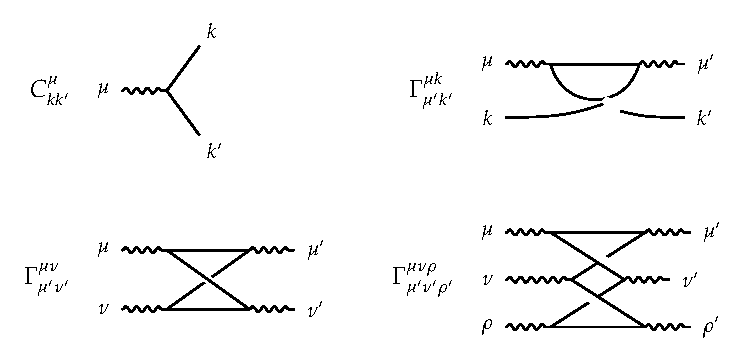
\includegraphics[width=0.8\textwidth]{pictures/9_1}
\par\end{centering}
\caption{\label{fig:9.1}物理量 $C$ 与 $\Gamma$ 的图形表示（此类图线并非附录 F 意义下的 Feynman
图）。}
\end{figure}

我们同样可以将多体 Hamiltonian（式 E.18）用集体费米子对算符 $b_{\mu}$ 与 $a_{\mu\nu}$
显式表示出来：
\begin{align}
H^{11} & =\sum_{\mu\nu}E_{\mu\nu}a_{\mu\nu},\nonumber \\
H^{22} & =\sum_{\mu\nu}V^{22}_{\mu\nu}b^{\dagger}_{\mu}b_{\nu},\label{eq:9.32}\\
H^{31} & =\sum_{\mu\nu\rho}V^{31}_{\mu\nu\rho}b^{\dagger}_{\mu}a_{\nu\rho}+\text{h.c.},\nonumber \\
H^{40} & =\sum_{\mu\nu}V^{40}_{\mu\nu}b^{\dagger}_{\mu}b^{\dagger}_{\nu}+\text{h.c.},\nonumber 
\end{align}
其中的展开矩阵元为：
\begin{align}
E_{\mu\nu} & =\frac{1}{M-2}\sum_{k}\left(\Gamma^{\nu k}_{\mu k}-\frac{1}{M-1}\delta_{\mu\nu}\right)E_{k},\nonumber \\
V^{22}_{\mu\nu} & =\frac{1}{4}\sum_{klpq}H^{22}_{klpq}C^{\mu*}_{kl}C^{\nu}_{pq},\label{eq:9.33}\\
V^{31}_{\mu\nu\rho} & =\frac{1}{M-2}\sum_{klpq}H^{31}_{klpq}C^{\mu*}_{kl}\left(\Gamma^{\rho q}_{\nu p}-\frac{1}{M-1}\delta_{\rho\nu}\delta_{pq}\right),\nonumber \\
V^{40}_{\mu\nu} & =\sum_{klpq}H^{40}_{klpq}C^{\mu*}_{kl}C^{\nu*}_{pq}.\nonumber 
\end{align}
一个具有特殊重要性的物理实例是 \textbf{Lipkin 模型}（参见 \ref{sec:5.4_Lipkin=006A21=00578B}），后文中我们还将对此进行详尽探讨。在此，我们在准粒子表象下应用该模型：算符
$\alpha^{\dagger}_{m}=c^{\dagger}_{m}$（以及 $\beta^{\dagger}_{m}=c_{-m}$）分别对应于在上能级中产生一个粒子（以及在下能级中产生一个空穴）。在
Hartree-Fock 基态 $|0\rangle$ 中，下能级（包含 $\Omega$ 个单粒子态）被完全填满：
\begin{equation}
\alpha_{m}|0\rangle=\beta_{m}|0\rangle=0.\label{eq:9.34}
\end{equation}
Hamiltonian 与准自旋算符 $\boldsymbol{K}^{2}$（式 5.47）严格对易。只要我们将讨论限制在具有本征值
$K=\Omega/2$ 的子空间中，就只有单一的集体费米子对算符（式 9.24）：
\begin{equation}
b^{\dagger}=\frac{1}{\sqrt{\Omega}}K_{+}=\frac{1}{\sqrt{\Omega}}\sum_{m}\alpha^{\dagger}_{m}\beta^{\dagger}_{m},\label{eq:9.35}
\end{equation}
其粒子-空穴振幅为 $C_{mm'}=(1/\sqrt{\Omega})\delta_{mm'}$（$m>0$）。算符 \ref{eq:9.25}
与 $K_{0}$ 紧密相连：
\begin{equation}
a=\frac{1}{\Omega}\sum_{m}\left(\alpha^{\dagger}_{m}\alpha_{m}+\beta^{\dagger}_{m}\beta_{m}\right)=1+\frac{2}{\Omega}K_{0}.\label{eq:9.36}
\end{equation}
单粒子态总数为 $M=2\Omega$，相应的 $\Gamma$ 量（式 9.28a, b）由下式给出：
\begin{equation}
\Gamma^{(2)}=+\frac{2}{\Omega},\qquad\Gamma^{(3)}=-\frac{2}{\Omega^{2}},\qquad\Gamma^{(4)}=+\frac{2}{\Omega^{3}},\quad\ldots\label{eq:9.37}
\end{equation}
此时，对易代数 \ref{eq:9.27a} 精确对应于角动量代数。以 $b$ 与 $a$ 表达的模型 Hamiltonian（式
5.45）形式为：
\begin{equation}
H=-\frac{\epsilon}{2}\Omega+\frac{\epsilon}{2}\Omega a-\frac{V}{2}\Omega(b^{\dagger}b^{\dagger}+bb).\label{eq:9.38}
\end{equation}
根据 \ref{subsec:9.2.2_=0073BB=008272=005C55=005F00=007684=006982=005FF5}
的讨论，我们本可以直接写出算符 $a$ 与 $b$ 的玻色展开；然而，我们首先希望更深入地研究一般多体情形。

依照 Belyaev 和 Zelevinski 针对一般多体情形的处理方案 \cite{BZ62}，我们首先引入一组纯理想玻色子算符：
\begin{equation}
[B_{\mu},B^{\dagger}_{\mu'}]=\delta_{\mu\mu'},\qquad[B_{\mu},B_{\mu'}]=0,\label{eq:9.39}
\end{equation}
并将费米子对算符 $b^{\dagger}_{\mu}$ 和 $a_{\mu\nu}$ 在玻色子空间中的对应像按如下方式展开\footnote{下列展开拟设显然并非唯一，但假定费米子对算符 $b^{\dagger}_{\mu}$ 的作用使玻色子数增加 1，而 $a_{\mu\nu}$
的作用不改变玻色子数，是极其合理且符合物理直觉的。}：
\begin{align}
(b^{\dagger}_{\mu})_{B} & =\sum_{\rho}x^{(1)}_{\mu\rho}B^{\dagger}_{\rho}+\sum_{\rho\nu\lambda}x^{(3)}_{\mu\nu\rho\lambda}B^{\dagger}_{\nu}B^{\dagger}_{\rho}B_{\lambda}+\cdots,\label{eq:9.40a}\\
(a_{\mu\nu})_{B} & =y^{(0)}+\sum_{\rho\lambda}y^{(2)}_{\mu\nu\rho\lambda}B^{\dagger}_{\rho}B_{\lambda}+\cdots.\label{eq:9.40b}
\end{align}
展开系数 $x^{(i)}$ 和 $y^{(i)}$ 由严格满足对易关系 \ref{eq:9.27a} 的条件唯一确定。在文献中，为了实现这一目标发展出了两种主要方法：

\subsubsection{微扰玻色展开\label{subsubsec:9.2.3.1_=005FAE=006270=0073BB=008272=005C55=005F00}}

微扰玻色展开方法建立在存在“小参数”的基础之上，对易子代数逐阶得到满足。该方法最早由 Belyaev 和 Zelevinski 提出
\cite{BZ62}，其后 Marshalek 详细研究了其数学与物理特性 \cite{Ma71,MH72,Ma74}。在那些工作中，作者们主要关注耦合到良好角动量的费米子对算符。在那种情形下，“小参数”为：
\begin{equation}
\epsilon=\frac{1}{2\bar{j}+1},\label{eq:9.41}
\end{equation}
其中 $\bar{j}$ 是 Fermi 面附近各单粒子能级的平均角动量。在实际原子核中，这一参数通常并不非常小。然而，若像式 \ref{eq:9.24}
那样处理集体费米子对，该方法的表现将大大改善。正如我们将看到的，此时的“小参数”正是式 \ref{eq:9.28a} 中的物理量
$\Gamma^{\mu\rho}_{\nu\sigma}$。如果用于展开的玻色子确实具有高度的集体性——即如果展开系数 $C^{\mu}_{kl}$
包含大量量级微小的分量——则 $\Gamma^{(2)}$ 的数值就会变得极小。Lipkin 模型便是一个典型范例 {[}参见式
\ref{eq:9.37}{]}，在那里我们有 $\Gamma^{(2)}\propto\epsilon=1/\Omega$。在这些情形下，式
\ref{eq:9.28b} 中的高阶顶点 $\Gamma^{(3)},\Gamma^{(4)}$ 均为 $\epsilon^{2},\epsilon^{3},\ldots$
的更高阶小量。

对易代数 \ref{eq:9.27a} 的满足分两步实现。首先，通过直接应用关系式 \ref{eq:9.29} 或 \ref{eq:9.30}，我们可以证明子代数
\ref{eq:9.27e} 仅通过对式 \ref{eq:9.40b} 进行有限阶展开即可精确满足：
\begin{equation}
(a_{\mu\nu})_{B}=\sum_{\rho\sigma}\Gamma^{\mu\rho}_{\nu\sigma}B^{\dagger}_{\rho}B_{\sigma},\label{eq:9.42}
\end{equation}
即 $y^{(2)}_{\mu\nu\rho\lambda}=\Gamma^{\mu\rho}_{\nu\lambda}$，而所有其他高阶系数
$y^{(n)}$ 均严格恒等于零。在下一步中，我们尝试在 $\Gamma$ 的每一微扰阶数下满足式 \ref{eq:9.27b}。零阶给出
$x^{(1)}_{\mu\rho}=\delta_{\mu\rho}$；一阶由 $x^{(3)}_{\mu\nu\rho\sigma}=-\frac{1}{4}\Gamma^{\nu\rho}_{\mu\sigma}$
满足，依此类推。经过相当冗长但直接的推导（该结果在 \ref{subsec:9.2.6_=006570=005B66=0080CC=00666F}
中可以用极其简捷的方法获得），我们最终得到无限阶微扰级数展开：
\begin{equation}
(b^{\dagger}_{\mu})_{B}=B^{\dagger}_{\mu}-\frac{1}{4}\sum_{\rho\sigma\nu}\Gamma^{\nu\rho}_{\mu\sigma}B^{\dagger}_{\nu}B^{\dagger}_{\rho}B_{\sigma}+\frac{1}{16}\sum_{\substack{\nu\rho_{1}\sigma_{1}\\
\rho_{2}\sigma_{2}
}
}\Gamma^{\nu\rho_{2}\rho_{1}}_{\mu\sigma_{1}\sigma_{2}}B^{\dagger}_{\nu}B^{\dagger}_{\rho_{1}}B_{\sigma_{1}}B^{\dagger}_{\rho_{2}}B_{\sigma_{2}}+\cdots,\label{eq:9.43}
\end{equation}
它属于式 \ref{eq:9.40a} 的形式，其系数为：
\begin{equation}
x^{(2n+1)}_{\mu\nu\rho_{1}\sigma_{1}\rho_{2}\sigma_{2}\cdots\rho_{n}\sigma_{n}}=-\frac{1}{2}\binom{1/2}{n}\Gamma^{\nu\rho_{n}\rho_{1}\rho_{2}\cdots}_{\mu\sigma_{1}\sigma_{2}\cdots\sigma_{n}}.\label{eq:9.44}
\end{equation}
我们还可以验证，该表达式在每一阶上都严格满足式 \ref{eq:9.27c} 与 \ref{eq:9.27d} 的对易关系。以此方式获得的玻色展开式相对于玻色子真空而言并非正规序（normal
order）。

在推导这些表达式的过程中，我们在许多地方使用了系数 $C^{\mu}_{kl}$ 的完备性关系 \ref{eq:9.26} 以及形如式
\ref{eq:9.30} 的求和恒等式。这意味着原则上我们必须包含所有 $\mu$ 指标及其对应的 TDA 方程（式 8.10）的解。然而在这些解中，包含了大量非集体的玻色子，对于它们而言高阶项
$\Gamma^{(n)}$ 绝不会迅速衰减。因此，只有当我们自身局限在少数几个集体玻色子（由它们所张成的空间称为\textbf{集体子空间}）之内，并且系数
$\Gamma$ 具有不将这些集体玻色子与 Hilbert 空间其余部分显著混合的特性时，整个展开才具有物理意义。例如在 Lipkin
模型中 {[}参见式 \ref{eq:9.37}{]}，$SU(2)$ 对称性保证了集体子空间的完全解耦。但在一般核多体系统中，要想找到这样一个理想解耦的集体子空间并非易事。

另一方面，要求 $\Gamma$ 不引入集体子空间与其余空间的耦合仅仅是一项\textbf{运动学条件}，它只取决于底层玻色子基底的性质。单凭这一条件尚不足以保证玻色展开的物理合理性。正如引言所指出的，只有当体系的
Hamiltonian 在集体子空间与其余 Hilbert 空间之间不产生剧烈耦合时，限制在集体子空间才是合理的，亦即集体子空间必须在良好近似下包含体系的真实物理本征态。由于这一条件直接取决于
Hamiltonian 的结构，因此被称为\textbf{动力学条件}。

基于群论对称性原因，这两项条件有时能够同时得到满足。Lipkin 模型再次为此提供了范例，在其中我们可以严格限制在具有准自旋 $\Omega/2$
的集体子空间中。此时我们只有单一的玻色子 $B$，由式 \ref{eq:9.35} 与 \ref{eq:9.42} 可得：
\begin{align}
a & =\frac{2}{\Omega}B^{\dagger}B,\nonumber \\
b^{\dagger} & =B^{\dagger}-\frac{1}{2\Omega}B^{\dagger}B^{\dagger}B-\frac{1}{8\Omega^{2}}B^{\dagger}B^{\dagger}BB^{\dagger}B-\cdots,\label{eq:9.45}
\end{align}
该级数可以精确求和为：
\begin{equation}
b^{\dagger}=B^{\dagger}\sqrt{1-\frac{1}{\Omega}B^{\dagger}B}.\label{eq:9.46}
\end{equation}
这与准自旋算符 $K_{\pm},K_{0}$ 的 Holstein-Primakoff 表象（式 9.4）完全一致。因此，Belyaev-Zelevinski
的微扰玻色展开通常也被称为 Holstein-Primakoff 展开。若我们将 Hamiltonian（式 9.38）展开至 $1/\Omega$
阶，并在正规序下排列，便得到：
\begin{equation}
H_{B}=-\frac{\epsilon}{2}\Omega+\epsilon B^{\dagger}B-V\frac{\Omega}{2}\left[\left(1-\frac{1}{2\Omega}\right)B^{\dagger}B^{\dagger}-\frac{1}{\Omega}B^{\dagger}B^{\dagger}B^{\dagger}B+\text{h.c.}\right].\label{eq:9.47}
\end{equation}
微扰玻色展开的一大显著优势在于：在最低级近似下，它严格对应于第 8.4 节中的 RPA 近似。为了看清这一点，我们采用非集体玻色子算符，并在式
\ref{eq:9.43} 中截断至第一项，即：
\[
(\alpha^{\dagger}_{k}\alpha^{\dagger}_{l})_{B}=B^{\dagger}_{kl},\qquad(\alpha^{\dagger}_{k}\alpha_{l})_{B}=\sum_{p}B^{\dagger}_{kp}B_{lp}.
\]
将这些表达式代入多体 Hamiltonian（式 E.18），并仅保留至多包含 $B^{\dagger}B,B^{\dagger}B^{\dagger},BB$
的二次项，我们便精确重现了准粒子表象（式 8.200）下的 RPA Hamiltonian（式 8.90）：
\begin{align}
H=E_{\text{HF}} & +\sum_{\substack{k<l\\
k'<l'
}
}\left\{ (E_{k}+E_{l})\delta_{kk'}\delta_{ll'}+H^{22}_{klk'l'}\right\} B^{\dagger}_{kl}B_{k'l'}\nonumber \\
 & +4\sum_{\substack{k<l\\
k'<l'
}
}\left\{ H^{40}_{klk'l'}B^{\dagger}_{kl}B^{\dagger}_{k'l'}+\text{h.c.}\right\} .\label{eq:9.48}
\end{align}
借此，我们还能以一种极为简明的方式理解为何 RPA 方法能够严格保持体系的对称性 \cite{Ma74}。由于玻色展开（式 9.43）的构建保证了在每一微扰阶数下分别独立满足对易关系，因此对于满足
\begin{equation}
[A,B]=C\label{eq:9.49}
\end{equation}
的任意两个物理算符 $A,B$，我们均有：
\begin{equation}
[A^{(n)},B^{(1)}]+[A^{(n-1)},B^{(2)}]+\cdots+[A^{(1)},B^{(n)}]=C^{(n-1)},\label{eq:9.50}
\end{equation}
其中 $A^{(n)},B^{(n)},C^{(n)}$ 分别是算符 $A,B,C$ 的玻色子部分中包含 $n$ 个 $B$
或 $B^{\dagger}$ 算符的 $n$ 阶展开项。对于与 $H$ 对易的对称性算符 $P$，从式 \ref{eq:9.50}
在 $n=2$ 时\footnote{项 $H^{(1)}$ 对应于式 7.36 中的 $H^{20}$，已被假定为零。}可得：
\begin{equation}
[H^{(2)},P^{(1)}]=0,\label{eq:9.51}
\end{equation}
这正是零频模式 $P^{(1)}$ 所满足的 RPA 方程（式 8.104）。这一论证可以平庸地推广到玻色展开的高阶项。然而，该优势在实际中的实用性受到如下事实的限制：它只有在对易代数得到精确满足时才严格成立；在更高阶展开中，我们通常需要引入截断至少数集体玻色子等激进近似，这往往会破坏对称性的严格守恒。

在数学结构上，玻色子的 RPA Hamiltonian（式 9.48）与费米子的一般单粒子 Hamiltonian（式 7.59）具有完全相同的形式。二者均可通过
Bogoliubov 变换对角化 {[}式 7.1 与式 8.91；另见附录 E.5{]}，分别导出 HFB 方程（式 7.42）与
RPA 方程（式 8.70）。唯一的区别在于 HFB 方程是非线性的，包含了费米子四阶项（即两体相互作用）的一部分贡献。在式 \ref{eq:9.48}
中推进到玻色展开的高阶项时，我们可以仿照式 7.57 的步骤，将所要计及的所有高阶算符项相对于新的玻色子真空进行正规序重排。所有的二次项
$B^{\dagger}B,B^{\dagger}B^{\dagger},BB$ 均可化为依赖于玻色子密度的单玻色场形式（式 8.90）。这样我们就得到了\textbf{自洽随机相位近似}（self-consistent
random phase approximation, SCRPA）\cite{SE73,Ma76a}。

\begin{figure}[H]
\begin{centering}
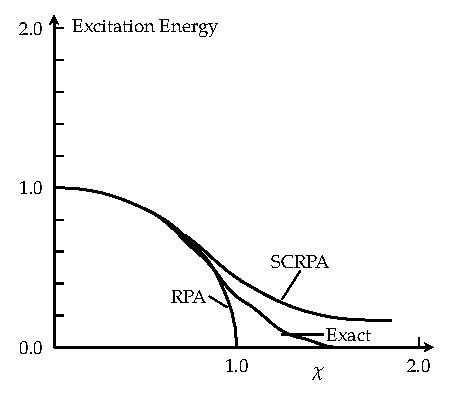
\includegraphics[width=0.7\textwidth]{pictures/9_2}
\par\end{centering}
\caption{\label{fig:9.2}自洽 RPA（SCRPA）与常规 RPA 以及 Lipkin 模型的精确解随相互作用强度参数 $\chi$
的变化对比（引自 \cite{SE73}）。}
\end{figure}

图 9.2 展示了该方法在 Lipkin 模型中的求解结果。我们可以极其清晰地看到，常规 RPA 在相变点区域的崩溃灾难（如 8.8.2
节所述）是如何通过计及玻色展开中的高阶项而得以完全避免的。当粒子数极其巨大时，SCRPA 与 RPA 逐渐趋于重合，这表明在宏观极限下可以出现严格的尖锐相变，而在有限核体系中，量子涨落总会在一定程度上将相变边界平滑地抹开（参见第
11 章）。

\subsubsection{限制在少数集体玻色子情形\label{subsubsec:9.2.3.2_=009650=005236=005728=005C11=006570=0096C6=004F53=0073BB=008272=005B50=0060C5=005F62}}

在某些具体核体系中，存在着充分的物理理由将动力学自由度限制在少数几个关键集体玻色子（如四极振动与配对振动）之内。此时，无限级数展开（式
9.43）通常不再能精确满足对易代数。追随 Sørensen 的构想 \cite{So67}，我们仍然可以采用截断至固定玻色子算符数目的拟设（式
9.40），并将展开参数 $x^{(1)},x^{(3)},\ldots,x^{(2n+1)}$ 以及 $y^{(0)},y^{(2)},\ldots,y^{(2n)}$
视为待定未知数。将该拟设直接代入对易代数中，通过计算对易子并令同类算符的展开系数彼此相等，我们便可获得一组关于系数 $x^{(i)}$
与 $y^{(i)}$ 的代数方程组（通常为非线性方程组）。例如在仅包含单一玻色子的情况下：
\begin{align}
1-y^{(0)} & =|x^{(1)}|^{2},\nonumber \\
-y^{(2)} & =2\left(|x^{(3)}|^{2}+x^{*}_{1}x_{3}+x^{*}_{3}x_{1}\right),\label{eq:9.52}\\
 & \;\;\vdots\nonumber 
\end{align}
求解这些方程组是完全可行的，Sørensen 将其计算推进至第四阶 \cite{So67,So68a,So68b,So69,So70,So71,So73}，而
Kishimoto 和 Tamura 则进一步在 Hamiltonian 中推进至第六阶 \cite{KT72,KT76}（另见
\cite{SP77b}）。然而，在方程组中常数参数 $y^{(0)}$ 始终是一个自由选取的开参数。改变该参数相当于在玻色子空间内部执行一次么正变换
\cite{So68b}。它对展开的收敛特性具有显著影响，并在文献中被以不同方式加以利用。

这种类型的玻色展开在本质上不再属于严格的微扰展开，因为当在拟设中计入更高阶项时，原有特定阶数上的系数数值也会随之发生修正。在此意义上，它能够更好地自适应于所考察的特定集体玻色子。至于
Hamiltonian 不应将集体子空间与 Hilbert 空间其余部分强烈耦合的动力学判据，在此类考量中依然必须得到严格遵守。

\subsection{Marumori 玻色展开\label{subsec:9.2.4_Marumori=0073BB=008272=005C55=005F00}}

Marumori 等人 \cite{MYT64a,MYT64b} 提出了一种从费米子空间到玻色子物理子空间态矢量的一一对应映射方法。该步骤最初是针对非集体玻色子给出的，我们将在
\ref{subsec:9.2.6_=006570=005B66=0080CC=00666F} 中对相关数学细节进行简要评述。由于在非集体情形下收敛性极差，Holzwarth
等人 \cite{LH75} 在实际计算中发展了一种采用少数集体玻色子的修正方案。该方法也已被成功应用于严格可解模型中 \cite{PKD68,KI69}。

从式 \ref{eq:9.24} 形式的集体费米子对算符 $b^{\dagger}_{\mu}$ 出发，我们引入归一化的 $2n$-费米子态：
\begin{equation}
|n\rangle=\mathscr{N}_{F}(n)|\mu_{1}\cdots\mu_{n}\rangle=\mathscr{N}_{F}(n)b^{\dagger}_{\mu_{1}}\cdots b^{\dagger}_{\mu_{n}}|0\rangle,\label{eq:9.53}
\end{equation}
其中 $\mathscr{N}_{F}(n)$ 是归一化常数。一般而言，这些态并不是彼此正交的。然而，只要仅计及少数几个集体算符且数目
$n$ 不是过大（即粒子总数不超过相应费米子空间的容纳限度），我们假定它们是线性独立的。其重叠范数矩阵 $N_{nn'}$ 定义为：
\begin{equation}
N_{nn'}=\langle\mu_{1}\cdots\mu_{n}|\mu'_{1}\cdots\mu'_{n'}\rangle.\label{eq:9.54}
\end{equation}
它与式 \ref{eq:9.28a} 中的量 $\Gamma$ 密切相关：
\begin{align}
N_{11}:\quad\langle\mu|\mu'\rangle & =\delta_{\mu\mu'},\nonumber \\
N_{22}:\quad\langle\mu\nu|\mu'\nu'\rangle & =\delta_{\mu\mu'}\delta_{\nu\nu'}+(\mu\leftrightarrow\nu)-\Gamma^{\mu\nu}_{\mu'\nu'},\label{eq:9.55}\\
N_{33}:\quad\langle\mu\nu\rho|\mu'\nu'\rho'\rangle & =\delta_{\mu\mu'}\delta_{\nu\nu'}\delta_{\rho\rho'}-\delta_{\rho\rho'}\Gamma^{\mu\nu}_{\mu'\nu'}-\Gamma^{\mu\nu\rho}_{\mu'\nu'\rho'}+(\text{若干对换项}).\nonumber 
\end{align}
对角矩阵元决定了归一化因子；例如对于双声子态的归一化因子，我们有：
\begin{equation}
\mathscr{N}_{F}(2)=\left(1+\delta_{\mu\nu}-\Gamma^{\mu\nu}_{\mu\nu}\right)^{-1/2}.\label{eq:9.56}
\end{equation}
Marumori 现在引入由归一化正交基底所张成的玻色子空间：
\begin{equation}
|n)=\mathscr{N}_{B}(n)|\mu_{1}\cdots\mu_{n})=\mathscr{N}_{B}(n)B^{\dagger}_{\mu_{1}}\cdots B^{\dagger}_{\mu_{n}}|0).\label{eq:9.57}
\end{equation}
其中 $\mathscr{N}_{B}$ 是形如 $(n_{1}!n_{2}!\cdots)^{-1/2}$ 的平庸组合因子（参见附录
C.19）。算符
\begin{equation}
U=\sum_{nn'}|n)N^{-1/2}_{nn'}\langle n'|\cdot\mathscr{N}^{-1}_{F}(n')\label{eq:9.58}
\end{equation}
将费米子空间映射到该玻色子空间中。在许多实际应用中（参见 \ref{subsec:9.2.8_=005E94=007528}），重叠矩阵
$N$ 是对角化的，否则算符 $N^{-1/2}$ 的作用即代表正交化过程。因此我们局限于此情形，并将物理算符变换到玻色子空间中：
\begin{equation}
H_{B}=UHU^{\dagger}=\sum_{nn'}\langle n|H|n'\rangle|n)(n'|.\label{eq:9.59}
\end{equation}
玻色子空间中的算符 $|n)(n'|$ 可以通过作用在玻色子真空上的投影算符来表达\footnote{双冒号 ${:}\cdots{:}$ 表示算符的正规乘积。式 \ref{eq:9.60} 的关系在单玻色子情形下极易直接证明：$B|0)(0|=B(1-B^{\dagger}B+\frac{1}{2}B^{\dagger}B^{\dagger}BB-\cdots)=B-B+B^{\dagger}BB-B^{\dagger}BB+\cdots=0$。}：
\begin{equation}
|0)(0|={:}\exp\left(-\sum_{\mu}B^{\dagger}_{\mu}B_{\mu}\right){:}=1_{B}-\sum_{\mu}B^{\dagger}_{\mu}B_{\mu}+\frac{1}{2!}\sum_{\mu\nu}B^{\dagger}_{\mu}B^{\dagger}_{\nu}B_{\mu}B_{\nu}-\cdots\label{eq:9.60}
\end{equation}
用显然的简记符号可以写为：
\begin{equation}
|n)(n'|=\mathscr{N}_{B}(n)\mathscr{N}_{B}(n')(B^{\dagger})^{n}\left(1-\cdots B^{\dagger}B+\cdots B^{\dagger}B^{\dagger}BB-\cdots\right)(B)^{n'}.\label{eq:9.61}
\end{equation}
如果 $|n\rangle$ 仅代表少数几个集体激发态，则 Hamiltonian（式 9.59）仅对应于多体 Hamiltonian
的集体部分，其本征态仅在全 Hamiltonian 不将集体子空间与 Hilbert 空间其余部分强烈耦合时才具有确定的物理意义。因此，合适玻色子的选择高度依赖于敏锐的物理直觉。

在式 \ref{eq:9.59} 中，集体 Hamiltonian 被表示为玻色子算符的正规序幂级数。它包含了多体 Hamiltonian
在集体子空间中的费米子矩阵元以及玻色子真空投影算符的展开式（式 9.60）。正如我们将看到的，在求和式 \ref{eq:9.59}
中通常仅需计及较小的 $n$ 和 $n'$ 值即可给出优良近似：$n+n'\le n_{\text{max}}$。因此，在实际应用中我们仅需要低阶的费米子矩阵元
$\langle n|H|n'\rangle$。这正是玻色子理论的核心实用优势。它们是在集体费米子对基底中、利用 Hamiltonian
的表象式 \ref{eq:9.32} 计算出来的。例如考虑矩阵元 $\langle n+2|H|n\rangle$，我们有：
\begin{equation}
\langle\mu_{1}\cdots\mu_{n+2}|H|\nu_{1}\cdots\nu_{n}\rangle=\sum_{\rho\sigma}V^{40}_{\rho\sigma}\langle\mu_{1}\cdots\mu_{n+2}|\rho\sigma\nu_{1}\cdots\nu_{n}\rangle.\label{eq:9.62}
\end{equation}
在假定 Hamiltonian 不散射出集体空间的条件下，对 $\rho$ 和 $\sigma$ 的求和被严格限制在少数几个集体指标之内，从而将问题归结为计算范数矩阵元（式
9.54）。这在实际计算中是一项相当繁复的工作，因为它们通过式 \ref{eq:9.28a} 中的 $\Gamma$ 量全面计入了
Pauli 原理的修正。

在此步骤中，人们通常采用一个额外的实用近似：若右侧对 $\rho$ 的求和仅遍历集体子空间中的态，则对易关系 \ref{eq:9.27c}
已经在集体空间内部得到了充分满足。这意味着双重对易子
\begin{equation}
\left[b_{\mu},[b_{\mu'},b^{\dagger}_{\nu'}]\right]=-\sum_{\rho}\Gamma^{\mu'\mu}_{\nu'\rho}b_{\rho}\label{eq:9.63}
\end{equation}
不会散射出集体空间之外；这一近似我们在 Belyaev-Zelevinski 理论中已经使用过。

利用式 \ref{eq:9.27b} 与 \ref{eq:9.27c}，我们随后可以导出范数矩阵元的递推关系 \cite{HJJ76,IST77,SP78}：
\begin{align}
\langle\mu_{1}\cdots\mu_{n}|\nu_{1}\cdots\nu_{n}\rangle & =\delta_{\mu_{1}\nu_{1}}\langle\mu_{2}\cdots\mu_{n}|\nu_{2}\cdots\nu_{n}\rangle\nonumber \\
 & \quad+\sum(\mu_{1}\text{ 与所有 }\mu_{2}\cdots\mu_{n}\text{ 对换})\nonumber \\
 & \quad-\sum_{\lambda}\Gamma^{\mu_{1}\mu_{2}}_{\nu_{1}\lambda}\langle\lambda\mu_{3}\cdots\mu_{n}|\nu_{2}\cdots\nu_{n}\rangle\nonumber \\
 & \quad-\sum\left[\mu_{1}\mu_{2}\text{ 与 }(\mu_{1}\cdots\mu_{n})\text{ 中的所有指标对对换}\right].\label{eq:9.64}
\end{align}
从双声子范数（式 9.55）出发，我们因而能够用 $\Gamma^{(2)}$ 表达所有的高阶范数矩阵元。Holzwarth 等人
\cite{HJJ76} 在实际过渡核中检验了该近似的可靠性，发现它与严格的范数矩阵元极其吻合。

我们将在 \ref{subsec:9.2.6_=006570=005B66=0080CC=00666F} 中看到，量 $\langle\mu_{1}\cdots\mu_{n}|\nu_{1}\cdots\nu_{n}\rangle$
正比于投影算符 $\hat{P}$ 在物理子空间中的矩阵元（参见式 9.99）。它们确切地反映了集体双准粒子算符 $b^{\dagger}_{\mu}$
并非真正玻色子这一事实。由这些算符张成的费米子空间是有限维的，而由相应玻色子算符张成的玻色子空间则是无限维的。因此，我们发现费米子范数与玻色子范数的商：
\begin{equation}
\nu(n)=\frac{\langle\mu_{1}\cdots\mu_{n}|\mu_{1}\cdots\mu_{n}\rangle}{(\mu_{1}\cdots\mu_{n}|\mu_{1}\cdots\mu_{n})}\label{eq:9.65}
\end{equation}
对于较大的 $n$ 值迅速跌落至极小。这意味着有效的费米子空间由于 Pauli 原理的压低而被急剧截断。特别地，我们发现耦合不同玻色子数状态的
Hamiltonian 矩阵元 $\langle n+2|H|n\rangle$ 随着 $n$ 的增大而迅速衰减。结果，我们完全可以将式
\ref{eq:9.59} 中的求和截断在很低的 $n$ 和 $n'$ 上。在很多实际问题中 \cite{HJJ76,SP77c}，将
Hamiltonian 的 Marumori 展开保留至四阶或六阶就已经是一种极高精度的优良近似。

总结上述结果，集体 Marumori 展开的有效性建立在两项先决条件之上：
\begin{enumerate}
\item \textbf{运动学条件}（纯粹与集体算符 $b^{\dagger}_{\mu}$ 及 $\Gamma$ 有关）：费米子范数矩阵元必须随着
$n$ 的增加而剧烈下降，从而使高阶项被 Pauli 原理有效截断；
\item \textbf{动力学条件}（与多体 Hamiltonian $H$ 的微观性质有关）：所选取的矢量 $|\mu_{1}\cdots\mu_{n}\rangle$
所张成的集体子空间必须与体系的真实本征子空间高度吻合，即 $H$ 与 Hilbert 空间其余部分的耦合必须极其微弱。
\end{enumerate}
第一项条件表面上似乎与微扰玻色展开中要求高度集体玻色子与微小 $\Gamma$ 值的条件（参见 \ref{subsubsec:9.2.3.1_=005FAE=006270=0073BB=008272=005C55=005F00}）相矛盾。对于微小的
$\Gamma$ 值，有效的费米子空间实际上相当庞大。事实上，第一项条件对于少数纯双准粒子算符而言满足得最好，因为此时有效费米子空间极小。然而在这种极端情况下，第二项动力学条件却几乎无法满足。只有对于真正的集体玻色子，相应的费米子空间才足够丰富，从而允许我们找到体系精确本征态能够被充分逼近的物理情形。事实证明，在这些情况下
Pauli 原理的压低效应依然足够强大，足以保证级数展开的迅速收敛 \cite{HJJ76}。

作为具体示范，我们再次考察 \ref{sec:5.4_Lipkin=006A21=00578B} 中的 Lipkin 模型（详细讨论参见
\cite{PKD68}）。根据式 \ref{eq:9.37} 与 \ref{eq:9.64}，我们得到范数的递推关系：
\begin{equation}
\langle(b)^{n}(b^{\dagger})^{n}\rangle=\langle(b)^{n-1}(b^{\dagger})^{n-1}\rangle\left[n-\frac{n}{2}(n-1)\frac{2}{\Omega}\right],\label{eq:9.66}
\end{equation}
该式在 Lipkin 模型中是严格成立的。对于归一化因子，它给出：
\begin{equation}
\mathscr{N}_{F}(n)=\sqrt{\frac{(\Omega-n)!}{\Omega!n!}\Omega^{n}},\qquad\mathscr{N}_{B}=\frac{1}{\sqrt{n!}}.\label{eq:9.67}
\end{equation}
根据式 \ref{eq:9.59}，保留至四玻色子项的 Hamiltonian（式 9.38）具有如下形式：
\begin{align}
H_{B}=-\frac{\epsilon}{2}\Omega+\epsilon B^{\dagger}B & -V\frac{\Omega}{2}\left[\sqrt{1-\frac{1}{\Omega}}B^{\dagger}B^{\dagger}\right.\nonumber \\
 & \quad\left.-\left(\sqrt{1-\frac{1}{\Omega}}-\sqrt{\left(1-\frac{1}{\Omega}\right)\left(1-\frac{2}{\Omega}\right)}\right)B^{\dagger}B^{\dagger}B^{\dagger}B+\text{h.c.}\right].\label{eq:9.68}
\end{align}
我们看到，Marumori 表象并不对应于 $1/\Omega$ 的渐近展开。每一个展开系数都内含了 $1/\Omega$ 的所有阶贡献。若将这些平方根按
$1/\Omega$ 展开到某一固定阶数，就能完全恢复出与 Belyaev-Zelevinski 展开等价的各项（式 9.47）。反之，通过对
Belyaev-Zelevinski 展开的所有阶项进行正规序重排，并对属于固定玻色子数目的算符系数进行全面求和，也能够精确导出 Marumori
Hamiltonian，因为两种展开在无穷阶意义下是严格等价的（参见 \ref{subsec:9.2.6_=006570=005B66=0080CC=00666F}）。Marumori
展开的不可替代的优势在于：它在每一个有限阶数 $n$ 上都严格计入了 Pauli 原理。

事实上，将 Marumori 算符在至多包含 $N_{\text{max}}$ 个玻色子的截断玻色子空间中对角化，精确等价于将费米子
Hamiltonian 在由费米子态 $|n\rangle$（$n\le N_{\text{max}}$）所张成的子空间中对角化。在后一种做法中，我们必须显式计算费米子矩阵元
$\langle n|H|n'\rangle$。从式 \ref{eq:9.59} 可以看出，这些量正是 Marumori 算符在玻色子空间中的矩阵元
$(n|H_{B}|n')$。转录到玻色子图象的优越性在于：在上述物理条件下，对 $n$ 的求和可以安全地限制在一个很小的上限
$n_{\text{max}}$ 上。这意味着高阶矩阵元 $(n|H_{B}|n')$ 可以完全用仅包含低阶费米子矩阵元的求和式表达出来。

若我们计入所有的费米子对 $b^{\dagger}_{\mu}$（包括所有的非集体对），Marumori 方法就精确对应于在 $2N_{\text{max}}$-准粒子空间中的壳模型组态相互作用计算。因此在最低阶近似下，我们得到的不是
RPA，而是 TDA 近似。

\subsection{Dyson 玻色展开\label{subsec:9.2.5_Dyson=0073BB=008272=005C55=005F00}}

迄今为止所讨论的玻色子表象都是无穷阶级数展开，它们仅在某些特定物理条件（例如底层费米子对具有极高集体性）下才具有良好的收敛性。在某些情况下——尤其是紧邻闭壳层的核体系中——我们必须显式计及其他集体性较弱的双费米子对及其与集体子空间的相互混合。在这些情形下，我们必须允许引入多种具有不同集体性程度的玻色子。尽管如此，人们依然希望至少对于核体系的低激发态，展开能够关于不同类型玻色子的数目
$m$ 迅速收敛。

这代表了一种截然不同的收敛类型（即图 9.3 中的垂直方向）。借助 Dyson 的玻色子表象，人们能够系统地研究这一问题，因为该方法最终给出一个严格有限阶截断的玻色子
Hamiltonian。图 9.3 同时也标明了迄今为止文献中所探讨的几类典型物理情形。在软核的过渡区中，人们检验了包含少数几个集体玻色子的水平方向收敛性
\cite{HJJ76}；而在幻核 $^{208}\text{Pb}$ 的邻域中，人们则检验了针对许多不同类型玻色子（但每次仅激发少数几个声子）的垂直方向收敛性
\cite{IRS80}。

一般而言，体系很可能在某些状态下既需要激发许多不同类型的玻色子，又需要激发同一类型的多个声子；这一极端复杂的区域在图 9.3 中用问号标出，至今仍是理论处理上的前沿挑战。

\begin{figure}[H]
\begin{centering}
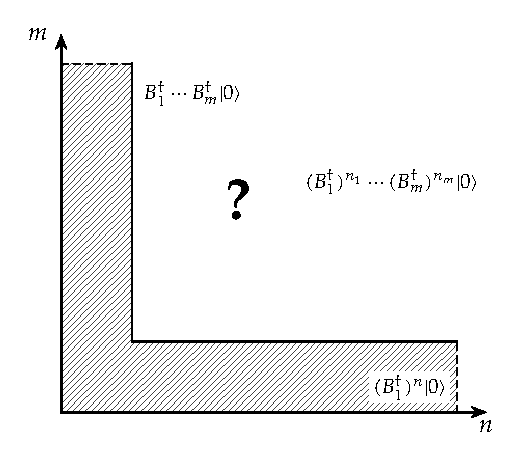
\includegraphics[width=0.7\textwidth]{pictures/9_3}
\par\end{centering}
\caption{\label{fig:9.3}玻色展开中所面临的两种收敛类型的示意图。$m$ 给出了不同玻色子类型的数目 $B^{\dagger}_{1}\cdots B^{\dagger}_{m}$，而
$n$ 给出了同一类型玻色子的激发数目 $(B^{\dagger}_{1})^{n}$。}
\end{figure}

Dyson 表象建立在如下数学事实之上：通过引入非厄米映射，对易子代数 \ref{eq:9.27a} 可以通过如下严格有限的变换精确满足\footnote{该表象的早期版本形式，另见 \cite{Am67}。}
\cite{RS77a}：
\begin{align}
b^{\dagger}_{\mu}\to\tilde{B}^{\dagger}_{\mu} & =B^{\dagger}_{\mu}-\frac{1}{2}\sum_{\nu\rho\sigma}\Gamma^{\nu\rho}_{\mu\sigma}B^{\dagger}_{\nu}B^{\dagger}_{\rho}B_{\sigma},\label{eq:9.69a}\\
b_{\mu}\to B_{\mu},\label{eq:9.69b}\\
a_{\mu\nu}\to\sum_{\rho\sigma}\Gamma^{\mu\rho}_{\nu\sigma}B^{\dagger}_{\rho}B_{\sigma}.\label{eq:9.69c}
\end{align}
这是角动量代数的 Dyson 表象（式 9.9）向多体问题的直接推广。通过将费米子真空 $|0\rangle$ 映射为玻色子真空
$|0)$，我们便得到了 Hilbert 空间中态矢量的相应表示。

利用式 \ref{eq:9.32} 与 \ref{eq:9.69a} 的严格有限表达式，我们导出了一个有限截断的玻色子 Hamiltonian，它最高仅包含算符
$B$ 与 $B^{\dagger}$ 的六阶项。算符 $H^{11}$ 与 $H^{22}$ 保持玻色子数守恒。假定展开系数
$C^{\mu}_{kl}$ 由 TDA 方程（式 8.10）所确定，经过直接推导可得：
\begin{equation}
V^{22}_{\mu\nu}=\delta_{\mu\nu}\Omega_{\mu}-\sum_{k}\Gamma^{\mu k}_{\nu k}E_{k},\label{eq:9.70}
\end{equation}
以及
\begin{equation}
H^{11}+H^{22}=\sum_{\mu}\Omega_{\mu}B^{\dagger}_{\mu}B_{\mu}+\frac{1}{4}\sum_{\mu\nu\rho\sigma}W_{\mu\nu\rho\sigma}B^{\dagger}_{\mu}B^{\dagger}_{\nu}B_{\rho}B_{\sigma},\label{eq:9.71}
\end{equation}
其中的相互作用矩阵元为：
\begin{equation}
W_{\mu\nu\rho\sigma}=\sum_{klpq}C^{\mu*}_{kl}C^{\nu*}_{pq}C^{\rho}_{kp}C^{\sigma}_{lq}(E_{k}+E_{l}+E_{p}+E_{q}-\Omega_{\rho}-\Omega_{\sigma}).\label{eq:9.72}
\end{equation}
Hamiltonian 中的其余项破坏玻色子数守恒，其显式形式可在文献 \cite{RS77a} 中找到。

Dyson 表象的一个显著缺点在于它破坏了 Hermite 性，这从式 \ref{eq:9.71} 中的有效相互作用 $W$ 便可清晰看出。态矢与左矢在玻色子空间中的对应像为：
\[
|\mu_{1}\cdots\mu_{n}\rangle\to\tilde{B}^{\dagger}_{\mu_{1}}\cdots\tilde{B}^{\dagger}_{\mu_{n}}|0),\qquad\langle\mu_{1}\cdots\mu_{n}|\to(0|B_{\mu_{n}}\cdots B_{\mu_{1}},
\]
它们彼此之间不再构成正交基底。与式 \ref{eq:9.54} 类似，重叠范数矩阵 $N$ 为：
\begin{equation}
N(\mu_{1}\cdots\mu_{n},\mu'_{1}\cdots\mu'_{n})=(0|B_{\mu_{1}}\cdots B_{\mu_{n}}\tilde{B}^{\dagger}_{\mu'_{1}}\cdots\tilde{B}^{\dagger}_{\mu'_{n}}|0).\label{eq:9.73}
\end{equation}
由于现代科学计算中存在针对大型非 Hermite 矩阵的高效对角化算法，因此这在实用中并不是致命障碍 \cite{RS74b,SWR76,Sch76}。我们将在
\ref{subsec:9.2.6_=006570=005B66=0080CC=00666F} 与 \ref{subsec:9.3.6_=004E2D=007B49=008026=005408=004E0EDyson=0073BB=008272=005C55=005F00}
中探讨其更深层次的数学细节。

如果能够合理忽略具有不同玻色子数目的子空间之间的相互耦合，该方法就会变得异常简捷。在那些情形下，有效 Hamiltonian 仅由
$H^{11}+H^{22}$ 所完全表征，并能够完全用 TDA 振幅 $C^{\mu}_{kl}$、TDA 本征激发能 $\Omega_{\mu}$
以及单准粒子能量 $E_{k}$ 显式解析表达。

\subsection{数学背景\label{subsec:9.2.6_=006570=005B66=0080CC=00666F}}

在本小节中，我们将系统探讨迄今为止所处理的各种玻色子表象的深层数学性质，从而厘清不同理论方法之间的内在数学联系。对于不深究这些高度专门化数学推导的读者，可以略过本节。受篇幅所限，我们无法在此给出所有漫长繁复的推导细节，相关步骤请读者参阅原始文献。

为了透彻理解玻色子表象的数学架构，使用“非集体”玻色子 $B_{kl}=-B_{lk}$ 是极其方便的。它们的指标精确对应于费米子对（式
9.22），并服从标准玻色子对易关系：
\begin{equation}
[B_{kl},B_{k'l'}]=0,\qquad[B_{kl},B^{\dagger}_{k'l'}]=\delta_{kk'}\delta_{ll'}-(k\leftrightarrow l).\label{eq:9.74}
\end{equation}
从多费米子空间的一组完备正交基底
\begin{equation}
|n\rangle=|k_{1}l_{1}\cdots k_{n}l_{n}\rangle=\alpha^{\dagger}_{k_{1}}\alpha^{\dagger}_{l_{1}}\cdots\alpha^{\dagger}_{k_{n}}\alpha^{\dagger}_{l_{n}}|0\rangle\label{eq:9.75}
\end{equation}
出发，我们可以在玻色子空间中定义相应的正交态矢集合 \cite{MYT64a}：
\begin{equation}
|n)=\frac{1}{\sqrt{(2n-1)!!}}\sum_{P}(-)^{P}B^{\dagger}_{k_{1}l_{1}}\cdots B^{\dagger}_{k_{n}l_{n}}|0),\label{eq:9.76}
\end{equation}
其中 $P$ 遍历指标 $k_{1}\ldots l_{n}$ 的所有能够给出新玻色子组合 $B^{\dagger}_{k_{1}l_{1}}\cdots B^{\dagger}_{k_{n}l_{n}}$
的置换（即 $B^{\dagger}_{12}B^{\dagger}_{34}$ 与 $B^{\dagger}_{34}B^{\dagger}_{21}$
仅被计入一次）；总项数为 $(2n)!/(n!2^{n})=(2n-1)!!$ 项。

式 \ref{eq:9.76} 中的态矢 $|n)$ 张成了玻色子空间的一个线性子空间，即所谓的\textbf{物理子空间}。正如我们将证明的，在这一子空间与原费米子空间之间存在着严格的一一对应关系。玻色子空间的其余部分则包含了形如
$B^{\dagger}_{k_{1}l_{1}}\cdots B^{\dagger}_{k_{n}l_{n}}|0)$ 但在指标
$k_{1}\ldots l_{n}$ 上未完全反对称化的状态，它们实质上破坏了 Pauli 原理。含有此类成分的状态会对物理算符的期望值产生虚假的赝态贡献。

Janssen 等人 \cite{JDF71} 证明，式 \ref{eq:9.76} 中的基态矢还可以写为如下优美形式：
\begin{align}
|n) & =\frac{1}{\sqrt{(2n-1)!!}}\langle0|\exp\left\{ \frac{1}{2}\sum_{kl}B^{\dagger}_{kl}\alpha_{l}\alpha_{k}\right\} \alpha^{\dagger}_{k_{1}}\alpha^{\dagger}_{l_{1}}\cdots\alpha^{\dagger}_{k_{n}}\alpha^{\dagger}_{l_{n}}|0\rangle|0)\label{eq:9.77}\\
 & =\frac{1}{\sqrt{(2n-1)!!}}\tilde{B}^{\dagger}_{k_{1}l_{1}}\cdots\tilde{B}^{\dagger}_{k_{n}l_{n}}|0),\label{eq:9.78}
\end{align}
其中引入了非集体 Dyson 算符（式 9.69a）：
\begin{equation}
\tilde{B}^{\dagger}_{kl}=B^{\dagger}_{kl}-\sum_{pq}B^{\dagger}_{kp}B^{\dagger}_{lq}B_{pq}.\label{eq:9.79}
\end{equation}
作为示例，双玻色子基态显式为：
\begin{equation}
|2)=\frac{1}{\sqrt{3}}\tilde{B}^{\dagger}_{k_{1}l_{1}}\tilde{B}^{\dagger}_{k_{2}l_{2}}|0)=\frac{1}{\sqrt{3}}\left(B^{\dagger}_{k_{1}l_{1}}B^{\dagger}_{k_{2}l_{2}}-B^{\dagger}_{k_{1}k_{2}}B^{\dagger}_{l_{1}l_{2}}+B^{\dagger}_{l_{1}k_{2}}B^{\dagger}_{k_{1}l_{2}}\right)|0).\label{eq:9.80}
\end{equation}
投向物理子空间的投影算符 $\hat{P}$ 具有如下显式表达：
\begin{equation}
\hat{P}=\sum_{n}|n)(n|=\sum^{\infty}_{n=0}\frac{1}{(2n)!(2n-1)!!}\sum_{\substack{k_{1}\cdots k_{n}\\
l_{1}\cdots l_{n}
}
}\tilde{B}^{\dagger}_{k_{1}l_{1}}\cdots\tilde{B}^{\dagger}_{k_{n}l_{n}}|0)(0|\tilde{B}_{k_{n}l_{n}}\cdots\tilde{B}_{k_{1}l_{1}}.\label{eq:9.81}
\end{equation}
经过直接应用关系式
\begin{align}
\sum_{\substack{k_{1}\cdots k_{n}\\
l_{1}\cdots l_{n}
}
}\tilde{B}^{\dagger}_{k_{1}l_{1}}\cdots\tilde{B}^{\dagger}_{k_{n}l_{n}}|0)(0|\tilde{B}_{k_{n}l_{n}}\cdots\tilde{B}_{k_{1}l_{1}} & =(2n-1)!!\sum_{\substack{k_{1}\cdots k_{n}\\
l_{1}\cdots l_{n}
}
}\tilde{B}^{\dagger}_{k_{1}l_{1}}\cdots\tilde{B}^{\dagger}_{k_{n}l_{n}}|0)(0|B_{k_{n}l_{n}}\cdots B_{k_{1}l_{1}}\label{eq:9.82}
\end{align}
与
\begin{align}
(0|\tilde{B}_{p_{n}q_{n}}\cdots\tilde{B}_{p_{1}q_{1}}\tilde{B}^{\dagger}_{k_{1}l_{1}}\cdots\tilde{B}^{\dagger}_{k_{n}l_{n}}|0) & =(2n-1)!!(0|B_{p_{n}q_{n}}\cdots B_{p_{1}q_{1}}\tilde{B}^{\dagger}_{k_{1}l_{1}}\cdots\tilde{B}^{\dagger}_{k_{n}l_{n}}|0),\label{eq:9.83}
\end{align}
并定义算符
\begin{equation}
(B^{\dagger}B)_{kl}=\sum_{q}B^{\dagger}_{ql}B_{qk},\qquad\hat{N}=\frac{1}{2}\sum_{kl}B^{\dagger}_{kl}B_{kl},\label{eq:9.84}
\end{equation}
我们可以证明投影算符具有下列核心代数性质：
\begin{align}
[\hat{P},\tilde{B}^{\dagger}_{kl}] & =0,\qquad\hat{P}B_{kl}\hat{P}=B_{kl}\hat{P},\qquad[\hat{P},(B^{\dagger}B)_{kl}]=0,\label{eq:9.85}\\
\tilde{B}^{\dagger}_{kl}\hat{P} & =\hat{P}B^{\dagger}_{kl}(1+2\hat{N}),\qquad2\hat{P}B^{\dagger}_{kl}\hat{N}=-\hat{P}\left(B^{\dagger}\cdot(B^{\dagger}B)\right)_{kl}.\label{eq:9.86}
\end{align}
将费米子空间映射到玻色子物理子空间的方法有多种可能。Usui \cite{Us60} 引入了变换算符：
\begin{equation}
\bar{U}=\langle0|\exp\left\{ \frac{1}{2}\sum_{kl}B^{\dagger}_{kl}\alpha_{l}\alpha_{k}\right\} |0).\label{eq:9.87}
\end{equation}
在费米子空间中插入完备系（式 9.75）并利用式 \ref{eq:9.77}，该算符可写作：
\begin{equation}
\bar{U}=\sum_{n}\sqrt{(2n-1)!!}\,|n)(n|.\label{eq:9.88}
\end{equation}
它显然不是么正算符。因此，我们必须定义其共轭映射算符：
\begin{equation}
\tilde{U}=\sum_{n}\frac{1}{\sqrt{(2n-1)!!}}\,|n\rangle(n|=\bar{U}^{\dagger}\left((2\hat{N}-1)!!\right)^{-1},\label{eq:9.89}
\end{equation}
其中 $\hat{N}$ 是玻色子数算符（式 9.84）。若 $1_{F}$ 是费米子空间的单位算符，则有：
\begin{equation}
\tilde{U}\bar{U}=1_{F},\qquad\bar{U}\tilde{U}=\hat{P}.\label{eq:9.90}
\end{equation}
费米子对算符（式 9.22）在这一变换下的映射行为如下：
\begin{align}
b^{\dagger}_{kl} & \to\bar{U}\alpha^{\dagger}_{k}\alpha^{\dagger}_{l}\tilde{U}=\tilde{B}^{\dagger}_{kl}\cdot\hat{P},\nonumber \\
b_{kl} & \to\bar{U}\alpha_{l}\alpha_{k}\tilde{U}=B_{kl}\cdot\hat{P},\label{eq:9.91}\\
a_{kl} & \to\bar{U}\alpha^{\dagger}_{l}\alpha_{k}\tilde{U}=(B^{\dagger}B)_{kl}\cdot\hat{P}.\nonumber 
\end{align}
该变换显然精确对应于 \ref{subsec:9.2.5_Dyson=0073BB=008272=005C55=005F00} 中所讨论的
Dyson 表象。相应的玻色子有效 Hamiltonian 具有如下形式：
\begin{equation}
\bar{U}H\tilde{U}=H_{B}\cdot\hat{P},\label{eq:9.92}
\end{equation}
其中
\begin{align}
H_{B} & =\sum_{k}E_{k}(B^{\dagger}B)_{kk}+\sum_{klpq}\left(H^{40}_{klpq}\tilde{B}^{\dagger}_{kl}\tilde{B}^{\dagger}_{pq}+H^{40*}_{klpq}B_{kl}B_{pq}\right)\nonumber \\
 & \quad+\sum_{klpq}\left(H^{31}_{klpq}\tilde{B}^{\dagger}_{kl}(B^{\dagger}B)_{qp}+H^{31*}_{klpq}(B^{\dagger}B)_{pq}B_{kl}\right)\nonumber \\
 & \quad+\frac{1}{4}\sum_{klpq}H^{22}_{klpq}\tilde{B}^{\dagger}_{kl}B_{pq}.\label{eq:9.93}
\end{align}
只要我们将波函数严格局限在物理子空间内，就可以安全地省去投影算符 $\hat{P}$，并直接求解 Schrödinger 方程：
\begin{equation}
H_{B}|\Psi)=E|\Psi).\label{eq:9.94}
\end{equation}
然而我们必须警惕：方程中不可避免地存在着源于破坏 Pauli 原理的非物理赝解（spurious solutions）$|\Psi_{s})$。由于
$\hat{P}$ 与 $H_{B}$ 并不对易，这些赝态解可能具有物理子空间的分量，即 $\hat{P}|\Psi_{s})\ne0$。为了识别它们，必须检验判据
$(1-\hat{P})|\Psi_{s})\ne0$。在通过限制集体玻色子数目来对本征值问题进行近似求解时，赝解可能会与真实物理态相互混杂。为此，将
Hamiltonian 进行如下分解通常极具启发意义：
\begin{equation}
H_{B}=H^{0}_{B}+V_{B},\label{eq:9.95}
\end{equation}
其中 $H^{0}_{B}=\sum_{k}E_{k}(B^{\dagger}B)_{kk}$。由式 \ref{eq:9.85}
可知，$H^{0}_{B}$ 与 $\hat{P}$ 严格对易。因此，方程 \ref{eq:9.94} 的物理真解也必定满足方程：
\begin{equation}
\left(H^{0}_{B}+\hat{P}V_{B}\right)|\Psi)=E|\Psi).\label{eq:9.96}
\end{equation}
将任意本征解分解为物理部分与赝态部分：$|\Psi)=\hat{P}|\Psi)+(1-\hat{P})|\Psi)$，我们看到其赝态部分必然是
$H^{0}_{B}$ 对应于本征值 $E$ 的本征矢量：
\begin{equation}
H^{0}_{B}(1-\hat{P})|\Psi)=E(1-\hat{P})|\Psi),\label{eq:9.97}
\end{equation}
即式 \ref{eq:9.96} 的所有非物理赝解均精确拥有 $H^{0}_{B}$ 的本征值：
\begin{equation}
E_{k_{1}}+E_{l_{1}}+E_{k_{2}}+E_{l_{2}}+\cdots\label{eq:9.98}
\end{equation}
由于 $H^{0}_{B}$ 最低阶的赝本征函数是形如 $B^{\dagger}_{12}B^{\dagger}_{12}|0)$
的双玻色子态，因此式 \ref{eq:9.96} 的最低赝解位于自由四准粒子能量处。这通常远高于所感兴趣的低激发集体谱区，因而式
\ref{eq:9.96} 的近似求解不会导致物理态与非物理态之间的严重混杂。

在实际应用中，从集体玻色子出发是极为明智的。Hamiltonian $H_{B}$ 的集体形式已经在 \ref{subsec:9.2.5_Dyson=0073BB=008272=005C55=005F00}
中推导出来。为了应用式 \ref{eq:9.96}，我们仅需要投影算符 $\hat{P}$ 的矩阵元。由式 \ref{eq:9.81}
可知，它们直接由范数矩阵元（式 9.54 或 9.73）给出：
\begin{align}
(\mu_{1}\cdots\mu_{n}|\hat{P}|\mu'_{1}\cdots\mu'_{n}) & =(0|B_{\mu_{1}}\cdots B_{\mu_{n}}\hat{P}B^{\dagger}_{\mu'_{1}}\cdots B^{\dagger}_{\mu'_{n}}|0)\nonumber \\
 & =\frac{1}{(2n-1)!!}\langle\mu_{1}\cdots\mu_{n}|\mu'_{1}\cdots\mu'_{n}\rangle.\label{eq:9.99}
\end{align}
一旦获得了式 \ref{eq:9.94} 或 \ref{eq:9.96} 的物理本征解，我们便可以通过将跃迁算符 $Q$ 变换到玻色子空间来计算其跃迁矩阵元：
\begin{equation}
\bar{U}Q\tilde{U}=Q_{B}\cdot\hat{P},\label{eq:9.100}
\end{equation}
并进而得出：
\begin{align}
\langle\Psi|Q|\Psi\rangle & =\langle\Psi|\tilde{U}\bar{U}Q\tilde{U}\bar{U}|\Psi\rangle=(\Psi|Q_{B}\hat{P}|\Psi)\nonumber \\
 & =(\Psi|Q_{B}|\Psi).\label{eq:9.101}
\end{align}
这雄辩地表明：只要确信波函数 $|\Psi)$ 不含赝态成分，我们就能完全在玻色子空间内部完成所有感兴趣物理量的计算，而根本无需重新变换回费米子空间。在实用中，这可以通过将范数矩阵（式
9.99）对角化并严格限制在具有非零本征值的子空间中来实现。

Marumori 通过引入严格的么正映射来规避非 Hermite 算符：
\begin{equation}
U=\sum_{n}|n)(n|=\left((2\hat{N}-1)!!\right)^{-1/2}\bar{U},\label{eq:9.102}
\end{equation}
并利用式 \ref{eq:9.91} 与 \ref{eq:9.86} 导出：
\begin{align}
b^{\dagger}_{kl} & \to U\alpha^{\dagger}_{k}\alpha^{\dagger}_{l}U^{\dagger}=\tilde{B}^{\dagger}_{kl}(1+2\hat{N})^{-1/2}\hat{P}=\hat{P}\left(B^{\dagger}\sqrt{1-B^{\dagger}B}\right)_{kl}\hat{P},\nonumber \\
b_{kl} & \to U\alpha_{l}\alpha_{k}U^{\dagger}=(1+2\hat{N})^{-1/2}\tilde{B}_{kl}\hat{P}=\hat{P}\left(\sqrt{1-B^{\dagger}B}\cdot B\right)_{kl}\hat{P},\label{eq:9.103}\\
a_{kl} & \to U\alpha^{\dagger}_{l}\alpha_{k}U^{\dagger}=\hat{P}(B^{\dagger}B)_{kl}\hat{P}.\nonumber 
\end{align}
在所有实际应用中，式 \ref{eq:9.102} 中的平方根都必须用 Taylor 级数替代。因此，即使限制在物理子空间内，Marumori
理论最终也会产生无穷级数展开。平方根展开的系数为 $(-)^{n}\binom{1/2}{n}$。因此，式 \ref{eq:9.103}
精确对应于式 \ref{eq:9.43} 中的微扰玻色展开。若推进至无穷阶，它与 Marumori 方法完全等价。后者是在正规序重排后获得的。截断在有限阶时，两种方法之间则存在细微差别
{[}例如在 Lipkin 模型中对比式 9.47 与式 9.68{]}。

我们还清楚地看到：在非集体玻色子情形下，$\sqrt{1-B^{\dagger}B}$ 的形式级数展开并不收敛 \cite{Ok74}。只有通过引入集体玻色子并对相应子空间进行适当的动力学解耦，才能实现
\ref{subsec:9.2.4_Marumori=0073BB=008272=005C55=005F00} 中所论述的快速收敛。

\subsection{基于 pp-玻色子的方法\label{subsec:9.2.7_=0057FA=004E8Epp-=0073BB=008272=005B50=007684=0065B9=006CD5}}

迄今为止，我们所讨论的各种方法都建立在 Fermi 面附近的玻色子基础之上。这些玻色子在良好近似下由粒子-空穴（ph）对或双准粒子对所给出。其自然的直接后果是，在所有这些方法中玻色子数都是不守恒的。相应的有效
Hamiltonian 包含了诸如 $B^{\dagger}B^{\dagger},B^{\dagger}B^{\dagger}B$
等破坏玻色子数守恒的非对角项。

现在我们从一种完全不同的进路出发，即从裸真空 $|-\rangle$（在实际计算中也可以是完全惰性的双闭壳核芯）出发，逐步添加耦合为近似玻色子的双粒子对。单
$j$-壳层中的 Cooper 对\footnote{这与我们用大写字母表示玻色子的惯例有所不同；式 9.104 中的 $S_{+}$ 与式 9.105 中的 $D^{\dagger}_{\mu}$
代表纯粹的集体费米子对。而另一方面，式 9.119 中的算符 $s^{\dagger}$ 和 $d^{\dagger}$ 则是纯粹的理想玻色子。}（式 6.3）便是一个典型例子：
\begin{equation}
S_{+}\propto\sum_{m}C^{00}_{jmj-m}a^{\dagger}_{jm}a^{\dagger}_{j-m},\label{eq:9.104}
\end{equation}
或者四极粒子对：
\begin{equation}
D^{\dagger}_{\mu}\propto\sum_{mm'}C^{2\mu}_{jmjm'}a^{\dagger}_{jm}a^{\dagger}_{jm'}.\label{eq:9.105}
\end{equation}
在 Seniority 方案（\ref{sec:6.2_Seniority=0065B9=006848}）中，我们可以将基态表示为
Cooper 对的乘积（式 6.19）：
\[
|0\rangle\propto(S_{+})^{N/2}|-\rangle,
\]
并通过将一个 $S_{+}$ 算符替换为 $D^{\dagger}_{\mu}$（式 6.27）来构建某些特定的激发态：
\begin{equation}
|2\mu\rangle\propto(S_{+})^{N/2-1}D^{\dagger}_{\mu}|-\rangle.\label{eq:9.106}
\end{equation}
在一般情况下，我们可以从集体双粒子对出发：
\begin{equation}
b^{\dagger}_{\tau}=\frac{1}{2}\sum_{kl}C^{\tau}_{kl}a^{\dagger}_{k}a^{\dagger}_{l},\label{eq:9.107}
\end{equation}
并应用前述各小节所讨论的方法之一来构建玻色子表象。由于体系的真实核子数是严格守恒的，因此在表象中现在仅出现保持玻色子数守恒的项。例如在
Dyson 方法中，我们得到一个有限截断的四阶玻色子 Hamiltonian {[}参见式 \ref{eq:9.71}{]}：
\begin{equation}
H_{B}=\sum_{\tau}\Omega_{\tau}B^{\dagger}_{\tau}B_{\tau}+\frac{1}{4}\sum_{\tau_{1}\tau_{2}\tau_{3}\tau_{4}}W_{\tau_{1}\tau_{2}\tau_{3}\tau_{4}}B^{\dagger}_{\tau_{1}}B^{\dagger}_{\tau_{2}}B_{\tau_{3}}B_{\tau_{4}}.\label{eq:9.108}
\end{equation}
这里的展开系数 $C^{\tau}_{kl}$ 现在是粒子-粒子（pp）TDA 振幅，而 $\Omega_{\tau}$ 则由相应的本征能量给出。在其他表象方法中，我们也会得到类似的
Hamiltonian（可能是无穷阶且保持 Hermite 性，但同样守恒玻色子数）。

该方法的局限性在于：在微观层面上，它仅能应用于具有极少数玻色子的情况，例如紧邻具有完全惰性核芯的幻核。对于远离幻数闭壳层的原子核，我们需要大量的
pp-玻色子，而这些玻色子相应的 $C^{\tau}_{kl}$ 系数原本是在完全惰性核芯的基底上确定的。对于包含大量价核子的体系，这一基底未必依然优良，正如我们在考虑用
$^{16}\text{O}$ 惰性核芯来描述 $^{208}\text{Pb}$ 邻近核这一极端例子时所能轻易想象的那样。因此，对于远离闭壳层的核，若将振幅严格局限在惰性核芯基底上，pp-玻色子描述可能不再有效。然而，我们可以尝试将振幅
$C^{\tau}_{kl}$ 视为可调节参数，并通过例如变分计算来加以确定。

另一方面，由大量玻色子构成的复杂组态通常只能借助群论方法来系统处理。迄今为止，人们主要探讨了唯象模型。在这些模型中，最著名的是 Arima
和 Iachello 的相互作用玻色子模型（$SU(6)$ 模型）\cite{AI75a,AI75b}。它包含两类玻色子：对应于式
\ref{eq:9.104} 中的 Cooper 对的 $s$ 玻色子，以及对应于式 \ref{eq:9.105} 中五个四极对的五个
$d$ 玻色子。该体系的 Hermite 的有效 Hamiltonian 仅包含至多四阶的玻色子数守恒项 {[}参见式 \ref{eq:9.119}{]}：
\[
s^{\dagger}s,\quad d^{\dagger}d,\quad d^{\dagger}d^{\dagger}dd,\quad s^{\dagger}s^{\dagger}ss,\quad d^{\dagger}d^{\dagger}ss,\quad d^{\dagger}d^{\dagger}ds+\text{h.c.}
\]
若忽略描述玻色子间相互作用的四阶项，我们便拥有一个由 $A/2$ 个 $s$ 玻色子的直积所构成的无微扰基态，以及若干 $s$
玻色子被 $d$ 玻色子取代的激发态。最初，该模型纯粹是建立在唯象基础之上引入的。然而对于具有配对加四极相互作用（式 4.141）的单
$j$-壳层，通过将 pp-费米子对映射到合适的玻色子表象上，该模型同样可以从微观角度获得坚实的理论证明 \cite{AOI77}。我们将在下一小节中详细讨论该模型的若干经典应用。

pp-玻色子的另一个典型范例是 \textbf{Schwinger 表象} \cite{BM78}。在单粒子基底中工作，其中 $a^{\dagger}_{m}$
与 $a^{\dagger}_{i}$ 分别在 Fermi 面的上方与下方产生粒子，我们可以引入两类玻色子：对应于产生粒子-空穴型
pp 对 $a^{\dagger}_{m}a^{\dagger}_{i}$（一个在 Fermi 面上，一个在 Fermi 面下）的
$B$ 玻色子 $B^{\dagger}_{mi}$；以及对应于产生全占据型 pp 对 $a^{\dagger}_{i}a^{\dagger}_{j}$（两个粒子均在
Fermi 面以下）的 $A$ 玻色子 $A^{\dagger}_{ij}$。这两类玻色子均为服从标准玻色对易关系的理想玻色子：
\begin{equation}
[B_{mi},B^{\dagger}_{m'i'}]=\delta_{mm'}\delta_{ii'},\qquad[A_{ij},A^{\dagger}_{i'j'}]=\delta_{ii'}\delta_{jj'}-\delta_{ij'}\delta_{ji'}.\label{eq:9.109}
\end{equation}
为了描述偶数体系，我们仅需要单体密度算符 $a^{\dagger}_{k}a_{l}$。它们按如下规则映射：
\begin{align}
a^{\dagger}_{m'}a_{m} & \to(a^{\dagger}_{m'}a_{m})_{B}=\sum_{i}B^{\dagger}_{m'i}B_{mi},\nonumber \\
a^{\dagger}_{i'}a_{i} & \to(a^{\dagger}_{i'}a_{i})_{B}=\sum_{j}A^{\dagger}_{ij}A_{i'j},\label{eq:9.110}\\
a^{\dagger}_{m}a_{i} & \to(a^{\dagger}_{m}a_{i})_{B}=\sum_{j}B^{\dagger}_{mj}A_{ij},\nonumber \\
a^{\dagger}_{i}a_{m} & \to(a^{\dagger}_{i}a_{m})_{B}=(a^{\dagger}_{m}a_{i})^{\dagger}_{B}.\nonumber 
\end{align}
该映射严格保持了密度算符 $a^{\dagger}_{k}a_{l}$ 的对易关系以及 Hermite 性，并且在玻色子空间中给出了严格有限的表达式。从对应于费米子裸真空的玻色子真空
$|-\rangle$ 出发：
\begin{equation}
A_{ij}|-\rangle=B_{mi}|-\rangle=0,\label{eq:9.111}
\end{equation}
我们可以通过如下条件在玻色子空间中构建 Hartree-Fock 基态 $|\Phi_{0})$：
\begin{equation}
(a^{\dagger}_{m}a_{m})_{B}|\Phi_{0})=0,\qquad[\delta_{ii'}-(a^{\dagger}_{i}a_{i})_{B}]|\Phi_{0})=0.\label{eq:9.112}
\end{equation}
这些条件由如下行列式态矢严格满足：
\begin{equation}
|\Phi_{0})=\frac{1}{\sqrt{N!}}\det A^{\dagger}|-\rangle=\frac{1}{\sqrt{N!}}\left|\begin{matrix}A^{\dagger}_{11} & \cdots & A^{\dagger}_{N1}\\
\vdots &  & \vdots\\
A^{\dagger}_{1N} & \cdots & A^{\dagger}_{NN}
\end{matrix}\right||-\rangle.\label{eq:9.113}
\end{equation}
激发的 ph 态可以通过相继作用算符 $(a^{\dagger}_{m}a_{i})_{B}$ 来构建。由式 \ref{eq:9.110}
可以看出，此类操作的效果正是将行列式 \ref{eq:9.113} 中的第 $i$ 列算符 $A^{\dagger}_{j}$
替换为 $B^{\dagger}_{mj}$ 列。

这一玻色子表象是角动量情形下 Schwinger 表象（式 9.11）的直接多体推广。与此类表象相伴随的内在问题是：我们引入了过多的玻色子算符。态
$|\Phi_{0})$ 以及由此构建的多粒子-多空穴态张成了玻色子物理子空间的一组基底。可以证明，算符
\begin{equation}
L_{ii'}=\sum_{j}A^{\dagger}_{ji}A_{ji'}+\sum_{m}B^{\dagger}_{mi}B_{mi'}=(A^{\dagger}A+B^{\dagger}B)_{ii'}\label{eq:9.114}
\end{equation}
当 $i\ne i'$ 时湮灭所有这些基态，而在 $i=i'$ 时使它们保持不变；换言之，在物理子空间中我们必须严格服从约束条件：
\begin{equation}
L_{ii'}=(A^{\dagger}A+B^{\dagger}B)_{ii'}=\delta_{ii'}.\label{eq:9.115}
\end{equation}
这精确对应于角动量情形下的约束式 \ref{eq:9.14}。同时引入玻色子算符 $A$ 与 $B$ 使得玻色子空间急剧扩张，结果导致出现一整类破坏约束条件
\ref{eq:9.115} 的全新非物理赝解。

原则上，我们可以利用约束条件 \ref{eq:9.115} 来完全消去算符 $A_{ij},A^{\dagger}_{ij}$。在形式上这可以通过记作
\begin{equation}
A\sim\sqrt{1-B^{\dagger}B}\label{eq:9.116}
\end{equation}
来完成。将该表达式代入式 \ref{eq:9.110}，我们在物理子空间中便重新回到了 Holstein-Primakoff 表达式（式
9.4）。详尽的数学分析表明，消去过程 \ref{eq:9.116} 精确对应于玻色子空间内部的一个正则变换 \cite{BM78}。

以完全类似的方式，我们也可以在 Arima 和 Iachello 的 $SU(6)$ 模型中消去 $s$ 玻色子。此时我们便得到了该模型的
Holstein-Primakoff 表象，它仅包含具有式 \ref{eq:9.116} 类型平方根因子的 $d$ 玻色子。以此种形式表述的
$SU(6)$ 模型最早由 Janssen 等人进行了深入探讨 \cite{JJD74}。

迄今为止，我们仅在粒子表象中探讨了 Schwinger 玻色子。在文献中，人们也曾尝试过在准粒子表象的基础上引入一般的 Schwinger
表象 \cite{YN76,MNY77,FYN77,Fu77}。

\subsection{应用\label{subsec:9.2.8_=005E94=007528}}

许多研究组已经将玻色展开方法成功应用于过渡区核的微观与唯象描述中，涵盖了从弱非谐振子、经由强非谐过渡，直至良好形变核中的纯转动极限。从本质上讲，我们必须区分两类主要工作：一类是\textbf{唯象方法}，它们直接参数化具有简明群论结构的玻色子有效
Hamiltonian；另一类则是\textbf{微观方法}，其中玻色子有效 Hamiltonian 中的全部参数均从底层微观费米子多体
Hamiltonian 中严格推导得出。

\subsubsection{唯象模型与相互作用玻色子模型\label{subsubsec:9.2.8.1_=00552F=008C61=006A21=00578B=004E0E=0076F8=004E92=004F5C=007528=0073BB=008272=005B50=006A21=00578B}}

我们可以直接用唯象玻色子算符来表达 Hamiltonian，而无需在细节上指定其深层微观费米子结构。取决于所包含的不同玻色子的类型数目以及展开截断的阶数，它包含若干待定参数
$h_{lm}$。一个典型范例是由保留至四阶的四极玻色子 $d^{\dagger}_{\mu}$ 所构成的体系（在此上下文中，“四极”一词仅仅意味着这些算符是
2 阶球面张量算符，并不指定相应费米子算符的径向波函数依赖性）：
\begin{align}
H=h_{00} & +h_{11}[d^{\dagger}d]_{0}+h_{20}[d^{\dagger}d^{\dagger}]_{0}+h_{30}[[d^{\dagger}d^{\dagger}]_{2}d^{\dagger}]_{0}+h_{21}[[d^{\dagger}d^{\dagger}]_{2}d]_{0}\nonumber \\
 & +h_{40}[d^{\dagger}d^{\dagger}]_{0}[d^{\dagger}d^{\dagger}]_{0}+h_{31}[d^{\dagger}d^{\dagger}]_{0}[d^{\dagger}d]_{0}\nonumber \\
 & +\sum_{L=0,2,4}h^{L}_{22}[[d^{\dagger}d^{\dagger}]_{L}[dd]_{L}]_{0}.\label{eq:9.117}
\end{align}
方括号表示角动量的张量耦合。将此类算符对角化是一项高度非平庸的数学任务。人们通常计算其在多玻色子基底之间的矩阵元，并求解相应的久期矩阵。然而，只有借助底层
Hamiltonian 的深层群论对称性，才能将该矩阵的维数控制在可处理的限度之内。例如，四极玻色子服从 $SU(5)$ 群对称性，这在文献中已经得到了极其详尽的研究
\cite{WHG66,KPW68,WP68,KT71}。

唯象 Hamiltonian（式 9.117）的对角化给出了一组依赖于常数 $h_{lm}$ 的能谱。在计算电磁跃迁几率时，我们还需要包含额外参数的跃迁算符的玻色子表象。将所有这些参数与实验能级及跃迁数据进行拟合，便能严格检验所观测到的物理现象是否确实能够由相应的玻色子机制所主导。如果拟合成功，我们便能获得关于有效相互作用的大量关键物理信息。但另一方面，由于缺乏直接的微观微商支撑，我们必须保持高度审慎，因为如果自由参数足够多，有时完全不同的物理机制也可能给出看似相近的拟合效果。

此类唯象模型的最简单版本仅使用五个四极玻色子以及一个关于玻色子数对角的四阶耦合项。在这些简化情形下，人们能够相当满意地拟合不同四极多重态中具有最高角动量的能级分支
\cite{BTK65,DDK70,HR74,IA74}。为了精确描述多重态的其余低自旋能级成员，则必须采用形如式 \ref{eq:9.117}
的更加一般的拟设 \cite{KS62,GG71,HL72a}。

从玻色子产生和湮灭算符 $B,B^{\dagger}$ 出发，我们可以定义相应的广义坐标 $Q$ 与广义动量 $P$ {[}参见式
8.95{]}，并将 Hamiltonian 形式上分解为动能项与势能项：
\begin{equation}
H(P,Q)=\frac{1}{2M}P^{2}+V(Q).\label{eq:9.118}
\end{equation}
要求“质量参数”既不依赖于 $P$ 也不依赖于 $Q$，会在玻色子 Hamiltonian 的各项参数之间导出简明的代数关系 \cite{Ho71a}。在四极模型中，内禀坐标系下的势能取决于原子核的变形参数
{[}参见式 1.13{]}。图 9.4 展示了 $^{76}\text{Se}$ 核中作为 $\beta$ 函数的势能曲线以及相应的计算能谱。该玻色子
Hamiltonian 的各项参数是通过拟合四个唯象参数而确定的。

\begin{figure}[H]
\begin{centering}
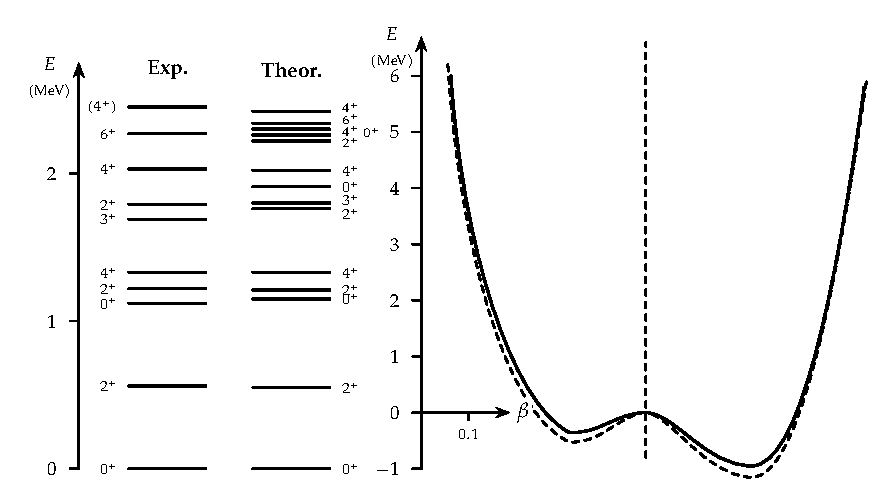
\includegraphics[width=0.75\textwidth]{pictures/9_4}
\par\end{centering}
\caption{\label{fig:9.4}$^{76}\text{Se}$ 的实验能级与唯象玻色子 Hamiltonian 本征值的对比。实线表示本征
$\beta\text{-}\gamma$ 坐标系在 $\gamma=0^{\circ}$ 时的势能曲线；虚线给出了源自微观自洽计算的势能曲线（引自
\cite{LH75}）。}
\end{figure}

通过在 Hamiltonian 中恰当选择参数，人们还能够平滑地描述从球形振动谱、经由中等非谐性、直至具有清晰转动能带结构的能谱相变演化
\cite{Ho70,GMG69,GMG70,DB70,GG71,Ho71a}。一旦有效势能 $V(Q)$ 具有极其深邃且明确的非零形变极小值，转动能带结构便会自然涌现（参见图
9.5）。然而在那些强烈形变的情形下，为了达到计算收敛，必须引入极其庞大数目的玻色子（多达 30 个声子）。除了高阶玻色子分量所带来的巨大数值计算开销之外，在物理层面上也难免令人产生深刻疑虑，因为如此庞大的声子数目极度强烈地违背了
Pauli 原理，而唯象 Hamiltonian 是否真正恰当地体现了这一基本量子禁戒在微观上是不清楚的。

多年来，核物理学界发展出了大量基于唯象群论技术的代数模型，它们的对角化借助成熟的李代数表示理论得到了极大的简化（参见例如 \cite{HNL70,DDK70,VNR75,RD76,RGB77}）。其中最著名、影响最深远的当属相互作用玻色子模型（Interacting
Boson Model, IBM，亦称 $SU(6)$ 模型），它最早由 Janssen 等人提出 \cite{JJD74}，随后由
Arima 和 Iachello 进行了极其系统深入的奠基性研究 \cite{AI75a,AI75b}。它的六个基本构件是五个具有角动量
2 的四极玻色子 $d^{\dagger}_{\mu}$（$\mu=-2,\ldots,+2$）和一个具有单态标量对称性的配对玻色子
$s^{\dagger}$。该模型保持总玻色子数严格守恒，属于 \ref{subsec:9.2.7_=0057FA=004E8Epp-=0073BB=008272=005B50=007684=0065B9=006CD5}
中所讨论的 Schwinger 类型的 pp-玻色子表象。其具有 Hermite 性的有效 Hamiltonian 形式如下：
\begin{align}
H=\epsilon_{s}s^{\dagger}s & +\epsilon_{d}[d^{\dagger}d]_{0}+\sum_{L=0,2,4}c_{L}[[d^{\dagger}d^{\dagger}]_{L}[dd]_{L}]_{0}+u_{0}s^{\dagger}s^{\dagger}ss\nonumber \\
 & +\left\{ v_{2}[[d^{\dagger}d^{\dagger}]_{2}[ds]_{2}]_{0}+v_{0}[d^{\dagger}d^{\dagger}]_{0}ss+u_{2}[[d^{\dagger}s^{\dagger}]_{2}[ds]_{2}]_{0}+\text{h.c.}\right\} .\label{eq:9.119}
\end{align}
它包含八个自由唯象参数 $\epsilon=\epsilon_{d}-\epsilon_{s},c_{0},c_{2},c_{4},u_{0},u_{2},v_{0},v_{2}$，这些参数通常由实验数据拟合确定。此外，我们还需要两个额外的耦合常数来定义电四极跃迁算符：
\begin{equation}
T_{2\mu}=q_{0}\left([d^{\dagger}s]_{2\mu}+\text{h.c.}\right)+q_{1}[d^{\dagger}d]_{2\mu}.\label{eq:9.120}
\end{equation}
在相互作用完全消失的平庸极限下（$c_{L}=v_{L}=u_{L}=0$），体系的基态纯粹由 $s$ 玻色子的凝聚所构成：
\[
|0)=\frac{1}{\sqrt{n!}}(s^{\dagger})^{n}|-\rangle,
\]
其中 $|-\rangle$ 代表裸真空，$2n$ 是核子总数。通过相继将一个或若干个 $s$ 玻色子替换为 $d$ 玻色子，我们在同一原子核中获得具有确定激发能量
$\epsilon=\epsilon_{d}-\epsilon_{s}$ 的四极集体激发态：
\[
|\mu)=\frac{1}{\sqrt{(n-1)!}}d^{\dagger}_{\mu}(s^{\dagger})^{n-1}|-\rangle.
\]
因此，其无微扰能谱展现为如图 1.5 所示的纯粹简谐四极多重态谱。继续添加更多的 $s$ 玻色子，我们便能如 Seniority
模型（参见 \ref{sec:8.2_Tamm-Dancoff=008FD1=004F3C}）所讨论的那样，自然跨越并描述具有核子数
$2n+2,2n+4,\ldots$ 的邻近偶偶核的能谱。

玻色子之间的相互作用项在体系中诱导了丰富的多体关联。此时必须在包含 $n_{s}$ 个 $s$ 玻色子与 $n_{d}=n-n_{s}$
个 $d$ 玻色子的多玻色子基底 $|n_{s},n_{d},\alpha)$ 中对角化 Hamiltonian（式 9.119）（$\alpha$
包含唯一确定该态所需的所有其余量子数）。利用群论张量代数方法，相关矩阵元的计算得到了极大的简化。

总玻色子数守恒关系式
\[
n=\hat{n}_{s}+\hat{n}_{d}=s^{\dagger}s+\sum_{\mu}d^{\dagger}_{\mu}d_{\mu}
\]
可被直接用于完全消去算符 $s$ 与 $s^{\dagger}$。对于固定的核子总数 $n$，基底态矢量完全由 $d$ 玻色子的量子数所表征，只要我们将湮灭算符
$s$ 形式替换为
\begin{equation}
s\to\sqrt{n-\sum_{\mu}d^{\dagger}_{\mu}d_{\mu}},\label{eq:9.121}
\end{equation}
便能严格保证 Hamiltonian 矩阵元的守恒。例如我们有：
\begin{align*}
s|n_{s}=n-n_{d},n_{d},\alpha) & =\sqrt{n_{s}}|n-n_{d}-1,n_{d},\alpha)\\
 & =\sqrt{n-\sum_{\mu}d^{\dagger}_{\mu}d_{\mu}}\,|n-n_{d}-1,n_{d},\alpha).
\end{align*}
将这一代换法则应用于算符（式 9.119），我们最终获得了一个仅包含四极玻色子 $d^{\dagger}_{\mu}$ 的有效 Hamiltonian。然而，它不再保持玻色子数守恒，并且通过对式
\ref{eq:9.121} 中的平方根进行 Taylor 展开，我们会得到包含无穷阶 $d^{\dagger}d\cdots$
的幂级数。这正是 $SU(6)$ 模型的 Holstein-Primakoff 版本 \cite{JJD74}。因此，引入 $s$
玻色子是一种极其精妙的代数工具，它通过将 Pauli 原理引入的非线性平方根因子代数化，巧妙地构建出了严格有限阶截断的代数玻色子表象。我们必须澄清的是：对于固定的粒子数而言，$s$
玻色子并没有引入任何新的物理自由度，它仅仅是用来构建无微扰基态的辅助算符；该模型并不包含 8.3.5 节所讨论的 $2p\text{-}2h$
类型的 $0^{+}$ 配对振动。另一方面，$s$ 玻色子的引入允许人们在一个统一的代数框架下系统处理相邻的 $A+2,A+4,\ldots$
原子核基态与激发态。

取决于模型参数的具体取值，相互作用玻色子模型拥有若干重要的动力学对称性极限，它们对应于 $SU(6)$ 的不同子群链分解 \cite{CCF79}，并且在很多情况下能够给出优美的解析严格解。这些代数对称极限在实际原子核的集体激发分类中扮演着极其关键的角色：
\begin{enumerate}
\item \textbf{Seniority 极限（$SU(2)$ 对称性）}：当 $c_{L}=v_{L}=0,u_{2}=0$（即完全切断与
$d$ 玻色子的耦合）时，我们精确重现了 \ref{sec:6.2_Seniority=0065B9=006848} 中所讨论的单
$j$-壳层的 Seniority 方案：
\[
H=\epsilon_{s}s^{\dagger}s+u_{0}s^{\dagger}s^{\dagger}ss=-GS_{+}S_{-},
\]
相应的准自旋算符为：
\[
S_{+}=\sqrt{\Omega}s^{\dagger}\sqrt{1-\frac{s^{\dagger}s}{\Omega}},
\]
且参数对应关系为 $u_{0}=-G,\epsilon_{s}=G\cdot\Omega$。
\item \textbf{振动极限（$SU(5)$ 对称性）} \cite{AI76}：在弱相互作用极限下（$u_{L}=0;v_{L},c_{L}\ll\epsilon_{d}-\epsilon_{s}$），体系展现出
$SU(5)$ 振动动力学对称性。此时 $s$ 玻色子不发挥动态作用，在极限情况下我们仅有相互作用四极玻色子（参见 \cite{BTK65,DDK70,IA74}）：
\begin{equation}
H=\sum_{\mu}\epsilon_{d}d^{\dagger}_{\mu}d_{\mu}+\sum_{L=0,2,4}c_{L}[[d^{\dagger}d^{\dagger}]_{L}[dd]_{L}]_{0}.\label{eq:9.122}
\end{equation}
其所有本征能级和跃迁几率均能以严格解析闭合形式显式给出。
\item \textbf{转动极限（$SU(3)$ 对称性）} \cite{AI78a}：若模型的各项参数之间满足特定比值关系，Hamiltonian（式
9.119）可以被改写为角动量与四极张量算符标量积的形式：
\begin{equation}
H=\epsilon\sum_{\mu}d^{\dagger}_{\mu}d_{\mu}-\kappa'[\boldsymbol{L}\cdot\boldsymbol{L}]_{0}-\kappa[\boldsymbol{Q}\cdot\boldsymbol{Q}]_{0},\label{eq:9.123}
\end{equation}
其中包含常数 $\epsilon,\kappa,\kappa'$，三个角动量算符分量
\[
L_{\mu}=\sqrt{10}[d^{\dagger}d]_{1\mu},
\]
以及五个内禀四极算符
\[
Q_{\mu}=d^{\dagger}_{\mu}s+s^{\dagger}d_{\mu}-\frac{\sqrt{7}}{2}[d^{\dagger}d]_{2\mu}.
\]
当 $\epsilon=\kappa'=0$ 时，我们得到了建立在 $SU(3)$ 李代数之上的纯转动极限。这是费米子体系中著名的
Elliott 模型 \cite{El58} 的玻色子推广，其优良群论性质在文献中被广泛探讨 \cite{Ha68,Ve68,JDJ75}。该极限精确再现了轴对称刚性转子的能谱规律（伴随简并的
$2^{+}_{\beta}$ 与 $2^{+}_{\gamma}$ 能级）：
\[
E(\lambda,\mu,K,L,M)=\frac{3}{4}(\kappa-\kappa')L(L+1)-\kappa\left[\lambda^{2}+\mu^{2}+\lambda\mu+3(\lambda+\mu)\right],
\]
其中 $(\lambda,\mu,K,L,M)$ 是 $SU(3)$ 群的一整套特征量子数。
\item \textbf{$\gamma$-非稳定软振子极限（$O(6)$ 对称性）} \cite{AI78b,CC78,CBP78}：在各大主壳层即将填满的末端，$SU(6)$
的另一个重要子群 $O(6)$ 在原子核低激发能谱的分类中发挥了举足轻重的作用。在此极限下，全部能级本征值同样能够以简洁的代数形式给出。在特定的物理极限下，其数学解与著名的完全
$\gamma$-软形变谐振子模型——即 Wilets-Jean 模型 \cite{WJ56,Me78}——完全重合。
\end{enumerate}
由于 $SU(6)$ 相互作用玻色子模型有机地熔铸了如此多深刻的微观集体物理效应，且拥有多达 11 个可调的有效相互作用参数，因此在拟合球形核、弱形变过渡核乃至强形变核的大量实验能谱与电磁跃迁时均取得了无可争辩的巨大成功
\cite{Ia77,AOI78,Ia78}。在单 $j$-壳层配对加四极相互作用框架下，人们也已经给出了该模型坚实的微观理论论证
\cite{OAI78}。然而，一个包含完整单核子自由度及其微观耦合的完备微观推导，至今仍然是核理论中极具挑战性的前沿课题。

\subsubsection{微观计算\label{subsubsec:9.2.8.2_=005FAE=0089C2=008BA1=007B97}}

尽管唯象玻色子模型在拟合实验能谱和电磁跃迁几率方面取得了令人瞩目的辉煌成功，但只要缺乏直接的微观微商，我们就永远无法在逻辑上排除如下担忧：这些模型是否仅仅是通过对若干自由参数的人工精细微调，从而在数学上“模拟”了某些与真正玻色子动力学毫不相干的其他微观物理机制。因此，在核多体玻色理论的构建中，最为根本的基石在于严格证明：进入玻色子有效
Hamiltonian 的全部展开参数，在原则上都可以从微观的多体相互作用 Hamiltonian 中自洽推导出来。

Lee 和 Holzwarth \cite{LH75} 率先将基于集体玻色子的 Marumori 方法（\ref{subsec:9.2.4_Marumori=0073BB=008272=005C55=005F00}）应用于具有相当纯粹四极结构的非谐核体系中。他们将表面
$\delta$ 相互作用（式 4.117）的微观多体 Hamiltonian 在角动量为 2 的 TDA 集体玻色子基底上展开至第四阶，发现计算得到的有效展开系数
$h_{lm}$（式 9.117）与实验拟合所得参数展现出了令人信服的高度一致性 \cite{HL72a}。图 9.4 中的虚线直观地展示了以此方式微观计算出的玻色子有效势能曲线
$V(Q)$。

B. Sørensen 广泛采用了 \ref{subsubsec:9.2.3.2_=009650=005236=005728=005C11=006570=0096C6=004F53=0073BB=008272=005B50=0060C5=005F62}
中所论述的 Belyaev-Zelevinski 截断代数方法。在系列经典文献中 \cite{So67,So68a,So68b,So69,So70}，他系统探讨了闭壳附近的配对振动模式以及过渡区原子核中的四极振动模式。他采用经过轻微唯象修正的配对加四极相互作用（式
4.141），将微观多体 Hamiltonian 推进至四阶展开，不仅在半定量层面上成功再现了这些原子核的核心物理特征，而且揭示了其微观演化规律。然而，在集体模式与非集体的双准粒子单粒子态之间的动力学耦合变得不可忽略的情形下，该方法遇到了一定困难。

更为完备与深刻的微观微商计算由 Kishimoto 和 Tamura 彻底完成 \cite{KT72,KT76}。除了标准的单极配对加四极相互作用之外，他们还在微观相互作用中显式引入了四极配对力（式
4.134），并在 $I=2$ 的集体玻色子分支上将微观 Hamiltonian 系统展开至第六阶。他们的深入研究揭示：在许多过渡核中，集体分支与非集体分支之间的耦合至关重要。为了微观处理这种混合，他们引入了
Feshbach 投影算符形式体系 \cite{Fe58,Fe62}，从而在集体子空间中导出了包含能量依赖性的重整化有效相互作用参数
$\tilde{h}_{lm}$。这些极其艰深复杂的微观自洽计算不仅在近球形振动核中，而且在复杂的过渡核乃至具有良好转动特征的强形变核中，均展现出了与实验能谱及跃迁几率异乎寻常的绝佳吻合。图
9.5 展示了稀土区钐（Sm）同位素链从球形向稳定形变过渡的相变过程的经典微观计算成果，表 9.1 则列出了相应的电四极跃迁及光谱四极矩的对比数据。

\begin{figure}[H]
\begin{centering}
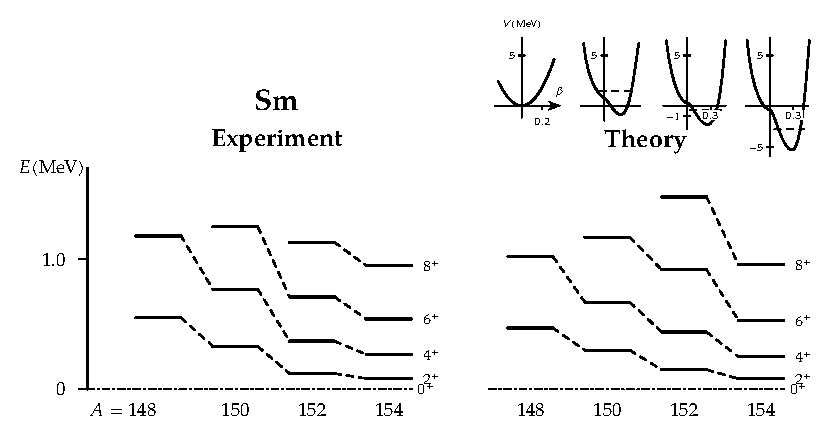
\includegraphics[width=0.85\textwidth]{pictures/9_5}
\par\end{centering}
\caption{\label{fig:9.5}钐（Sm）同位素核中从球形到形变的相变。能谱结构从纯振动态逐渐转变为规则的转动态。图中上方还给出了玻色子
Hamiltonian 随形变参数 $\beta$ 变化的相应微观有效势能曲线（引自 \cite{KT76}）。}
\end{figure}

\begin{table}[H]
\caption{\label{tab:9.1}利用微观玻色展开方法计算的第一激发 $2^{+}$ 态的光谱四极矩与 $B(E2)$ 跃迁值，并与实验测量数据进行对比（引自
\cite{TK73}）。}

\centering{}%
\begin{tabular}{|c|c|c|c|c|}
\hline 
 & \multicolumn{2}{c|}{$Q_{2^{+}}$ {[}$e\cdot\text{b}${]}} & \multicolumn{2}{c|}{$B(E2;2^{+}\to0^{+})$ {[}$e^{2}\cdot\text{b}^{2}${]}}\tabularnewline
\hline 
 & 实验值 & 理论值 & 实验值 & 理论值\tabularnewline
\hline 
$^{148}\text{Sm}$ & $-0.97\pm0.27$ & $-0.91$ & $0.141\pm0.005$ & $0.152$\tabularnewline
$^{150}\text{Sm}$ & $-1.31\pm0.19$ & $-1.17$ & $0.274\pm0.006$ & $0.270$\tabularnewline
$^{152}\text{Sm}$ & $-1.73\pm0.20$ & $-1.72$ & $0.666\pm0.014$ & $0.697$\tabularnewline
$^{154}\text{Sm}$ & $-1.91$ & $-1.91$ & $0.922\pm0.040$ & $0.884$\tabularnewline
\hline 
\end{tabular}
\end{table}


\section{奇 A 核与粒子-振动耦合\label{sec:9.3_=005947A=006838=004E0E=007C92=005B50-=00632F=0052A8=008026=005408}}

前文各节主要局限于由偶数个费米子所构成的原子核体系。显而易见，具有奇数质量数（奇 A）的原子核体系同样普遍存在着丰富的集体激发态。在核物理发展史上，最著名的代表性范例当属
$^{209}\text{Bi}$ 的微观七重态（septuplet）：在该核中，处于 $1h_{9/2}$ 单质子轨道上的奇价质子与双闭壳核芯
$^{208}\text{Pb}$ 在 $2.61\text{ MeV}$ 处的 $3^{-}$ 八极集体振动声子发生耦合。由于该奇质子对核芯集体振动仅产生极其微弱的微扰，从而在
$2.61\text{ MeV}$ 激发能附近诱导产生了一个能级劈裂极小（仅约数百 $\text{keV}$）的七重能级组态（角动量分别为
$3/2^{+},5/2^{+},7/2^{+},9/2^{+},11/2^{+},13/2^{+},15/2^{+}$；参见图
9.6）。在理论上，此类状态通常在粒子-振动耦合（particle vibration coupling, PVC，或 VPC）模型框架下处理
\cite{BM75}。事实表明，该模型在微观本质上与奇核系统的玻色展开方法紧密相连。

\begin{figure}[H]
\begin{centering}
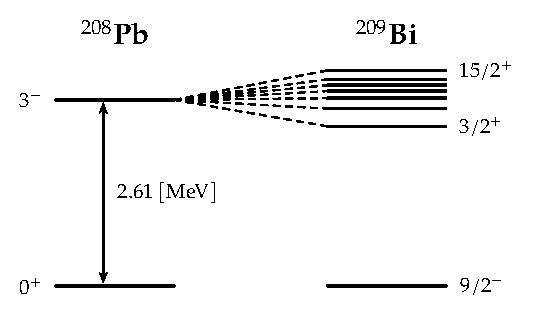
\includegraphics[width=0.7\textwidth]{pictures/9_6}
\par\end{centering}
\caption{\label{fig:9.6}$^{208}\text{Pb}$ 与 $^{209}\text{Bi}$ 实验激发能谱的示意性对比。}
\end{figure}


\subsection{奇 A 系统的玻色展开\label{subsec:9.3.1_=005947A=007CFB=007EDF=007684=0073BB=008272=005C55=005F00}}

前一节所考察的所有各类玻色子表象理论，均可系统推广至奇质量核体系 \cite{Ya65,DJ73,Ma73,Ma74,Pr74,RS77a,BM78}。由于其基本指导原则与偶偶核情形并无本质差异，在此我们仅简要勾勒
Belyaev-Zelevinski 方法与 Dyson 方法的核心框架。

在 Belyaev-Zelevinski 方法中，除了双费米子对算符 $b^{\dagger}_{\mu},a_{\mu\nu}$
{[}式 9.24 与式 9.25{]} 之外，我们现在还必须显式计入单费米子算符 $\alpha^{\dagger}_{k}$，并将所有这些算符统一映射到一个扩充的乘积空间中，即通常的
$B^{\dagger}_{\mu}$ 玻色子空间与由一个同玻色子完全对易的\textbf{理想费米子}（ideal fermion）$\beta^{\dagger}_{k}$
所张成的空间的直积：
\begin{equation}
[B_{\mu},\beta^{\dagger}_{k}]=[B^{\dagger}_{\mu},\beta^{\dagger}_{k}]=0.\label{eq:9.124}
\end{equation}
由于在同一时刻至多只允许存在一个理想费米子，因此算符 $\beta_{k}$ 满足代数关系 \cite{Ok74}：
\begin{equation}
\beta_{k}\beta_{l}=\beta^{\dagger}_{k}\beta^{\dagger}_{l}=0,\qquad\beta_{k}\beta^{\dagger}_{l}=\delta_{kl}.\label{eq:9.125}
\end{equation}
该扩充乘积空间中的真空投影算符由下式给出：
\begin{equation}
|0)(0|={:}\exp\left(-\sum_{\mu}B^{\dagger}_{\mu}B_{\mu}\right){:}\left(1-\sum_{k}\beta^{\dagger}_{k}\beta_{k}\right),\label{eq:9.126}
\end{equation}
这再次确切意味着：
\begin{equation}
B_{\mu}|0)=\beta_{k}|0)=0.\label{eq:9.127}
\end{equation}
于是，直积空间中的一组标准正交基底为：
\begin{equation}
|k,N)=\mathscr{N}_{B}\cdot\beta^{\dagger}_{k}B^{\dagger}_{\mu_{1}}\cdots B^{\dagger}_{\mu_{N}}|0),\qquad N=0,1,\ldots\label{eq:9.128}
\end{equation}
除了算符 $b^{\dagger}_{\mu}$ 与 $a_{\mu\nu}$ 的对易代数（式 9.27）之外，我们现在还必须考虑单费米子算符之间以及单费米子与对算符之间的反对易和对易关系：
\begin{align}
\{\alpha_{k},\alpha_{l}\} & =\{\alpha^{\dagger}_{k},\alpha^{\dagger}_{l}\}=0,\qquad\{\alpha_{k},\alpha^{\dagger}_{l}\}=\delta_{kl},\nonumber \\{}
[\alpha_{k},b_{\mu}] & =0,\qquad[\alpha_{k},b^{\dagger}_{\mu}]=\sum_{l}C^{\mu}_{kl}\alpha^{\dagger}_{l},\label{eq:9.129}\\{}
[\alpha_{k},a_{\mu\nu}] & =\sum_{l}\Gamma^{\mu k}_{\nu l}\alpha_{l},\nonumber 
\end{align}
其中 $\Gamma^{\mu k}_{\nu l}$ 由式 \ref{eq:9.29} 所定义。

现在我们仿照 \ref{subsubsec:9.2.3.1_=005FAE=006270=0073BB=008272=005C55=005F00}
的思路，对各物理算符在玻色子空间中的像做出如下展开拟设（选取该特定拟设形式的深入讨论参见 \cite{Ma74}）；在此我们只需指出，这些展开在微扰意义下逐阶精确满足上述对易规则\footnote{在非集体情形下，类似于式 9.103，我们可以对 $(b^{\dagger}_{kl})_{B}$ 与 $(\alpha^{\dagger}_{k})_{B}$
的无穷级数进行显式封闭求和：
\begin{align*}
(a_{kl})_{B} & =\sum_{r}B^{\dagger}_{lr}B_{kr}+\beta^{\dagger}_{l}\beta_{k},\\
(b^{\dagger}_{kl})_{B} & =\left(B^{\dagger}\sqrt{1-B^{\dagger}B}\right)_{kl}+\sum_{pq}\left[\left(\sqrt{1-B^{\dagger}B}\right)_{pq}B^{\dagger}_{kl}\right]\beta^{\dagger}_{p}\beta_{q},\\
(\alpha^{\dagger}_{k})_{B} & =\sum_{l}\left(\sqrt{1-B^{\dagger}B}\right)_{lk}\beta^{\dagger}_{l}+B^{\dagger}_{kl}\beta_{l}.
\end{align*}
}：
\begin{align}
(a_{\mu\nu})_{B} & =\sum_{\rho\sigma}\Gamma^{\mu\rho}_{\nu\sigma}B^{\dagger}_{\rho}B_{\sigma}+\sum_{kl}\Gamma^{\mu k}_{\nu l}\beta^{\dagger}_{k}\beta_{l},\nonumber \\
(b^{\dagger}_{\mu})_{B} & =B^{\dagger}_{\mu}-\frac{1}{4}\sum_{\nu\rho\sigma}\Gamma^{\nu\rho}_{\mu\sigma}B^{\dagger}_{\nu}B^{\dagger}_{\rho}B_{\sigma}+\cdots-\frac{1}{2}\sum_{\nu kl}\Gamma^{\nu k}_{\mu l}B^{\dagger}_{\nu}\beta^{\dagger}_{k}\beta_{l}+\cdots,\label{eq:9.130}\\
(\alpha^{\dagger}_{k})_{B} & =\beta^{\dagger}_{k}-\frac{1}{2}\sum_{\rho\sigma l}\Gamma^{\rho l}_{\sigma k}B^{\dagger}_{\rho}B_{\sigma}\beta^{\dagger}_{l}+\cdots+\sum_{\rho l}C^{\rho}_{kl}B^{\dagger}_{\rho}\beta_{l}.\nonumber 
\end{align}
借助这些算符展开式，我们便能直接构建出多体微观 Hamiltonian（式 9.32）在直积空间中的玻色子-费米子对应像。

\subsection{粒子-振动耦合（Bohr）Hamiltonian 的推导\label{subsec:9.3.2_=007C92=005B50-=00632F=0052A8=008026=005408Hamiltonian=007684=0063A8=005BFC}}

将式 \ref{eq:9.130} 代入 Hamiltonian（式 9.32 与 9.33）中，如果我们暂时忽略基态关联（即假定
$H^{40}=0$\footnote{由于忽略了 $H^{40}$，形如 $B^{\dagger}B^{\dagger}$ 与 $BB$ 的项暂时缺失。通过变换到
RPA 玻色子（参见附录 E.5），$B_{\mu}=\sum_{mi\rho}C^{\mu*}_{mi}(X^{\rho}_{mi}Q_{\rho}+Y^{\rho*}_{mi}Q^{\dagger}_{\rho})$，我们完全可以将它们自然计入。}），则在关于 $\Gamma$ 的一阶近似下可得：
\begin{align}
H & =\sum_{\mu}\Omega_{\mu}B^{\dagger}_{\mu}B_{\mu}+\sum_{k}E_{k}\beta^{\dagger}_{k}\beta_{k}+\cdots+H_{\text{coupl}},\nonumber \\
H_{\text{coupl}} & =\sum_{\mu,k,l}\frac{1}{2}\left(\gamma^{\mu}_{kl}B^{\dagger}_{\mu}\beta^{\dagger}_{k}\beta_{l}+\text{h.c.}\right)\label{eq:9.131}\\
 & \quad-\frac{1}{2}\sum_{\substack{\mu\nu\lambda\\
kl
}
}V^{22}_{\mu\nu}\left(\Gamma^{\lambda l*}_{\nu k}B^{\dagger}_{\mu}B_{\lambda}+\Gamma^{\lambda k}_{\mu l}B^{\dagger}_{\lambda}B_{\nu}\right)\beta^{\dagger}_{k}\beta_{l},\nonumber 
\end{align}
其中微观单粒子-振动耦合顶点定义为：
\begin{equation}
\gamma^{\mu}_{kl}=2\sum_{rs}H^{31}_{rskl}C^{\mu*}_{rs},\label{eq:9.132}
\end{equation}
这里的 $C^{\mu}_{rs}$ 是 TDA 振幅，$\Omega_{\mu}$ 是相应的本征能量。在式 \ref{eq:9.131}
中，我们略去了包含两个 $\Gamma$ 的 $B^{\dagger}B$ 项，因为它们通常远小于仅含单一 $\Gamma$
的主导项。耦合 Hamiltonian $H_{\text{coupl}}$ 中的第一项在核物理文献中被称为 \textbf{Bohr
耦合 Hamiltonian} \cite{BM75}，因为它最初是在唯象液滴模型中被推导出来的（参见 \ref{subsec:9.3.4_=007C92=005B50-=00632F=0052A8=008026=005408=009876=0070B9=007684=006027=008D28}）。而
$H_{\text{coupl}}$ 中的第二项则源自玻色展开的系统性微观推导，正如我们后文将阐明的，它在微观上精确起到了修正 Pauli
原理的作用。

对于具有时间反演不变性的多体系统，矩阵元 $H^{31}_{rskl}$ 可以在正则单粒子基底（参见第 7 章）中根据式 E.25
显式计算得出：
\begin{align}
H^{31}_{rskl}=\frac{1}{3}\cdot\frac{1}{4} & \left\{ -\bar{v}_{r\bar{k}\bar{s}l}\left(\eta^{+}_{rs}\xi^{+}_{kl}+\eta^{-}_{rs}\xi^{-}_{kl}\right)\right.\nonumber \\
 & \quad+\bar{v}_{sk\bar{r}l}\left(\eta^{+}_{rs}\xi^{+}_{kl}-\eta^{-}_{rs}\xi^{-}_{kl}\right)\label{eq:9.133}\\
 & \quad\left.+\bar{v}_{r\bar{s}\bar{k}l}\left(\xi^{+}_{rs}\eta^{+}_{kl}-\xi^{-}_{rs}\eta^{-}_{kl}\right)\right\} ,\nonumber 
\end{align}
其中占据因子 $\xi,\eta$ 的定义见式 8.202。

在下文中，我们将更加深入地考察不存在超流配对关联的核系统。此时，准粒子算符 $\beta^{\dagger}_{k}$ 必须替换为真实的单粒子产生算符
$c^{\dagger}_{m}$ 或单空穴产生算符 $c_{i}$（我们用指标 $m,n$ 表示粒子态，用 $i,j$ 表示空穴态；参见第
2 章）。准粒子能量相应地被单粒子能量 $\epsilon_{m}$ 或空穴能量 $-\epsilon_{i}$ 所替代（能量零点取为
$\epsilon_{F}=0$）。由于在一般的准粒子形式体系中我们既可以表示粒子-空穴振动（指标 $\nu,\nu',\ldots$），也可以表示粒子-粒子（或空穴-空穴）振动（指标
$\tau,\tau',\ldots$），因此我们自然获得两类耦合顶点。忽略配对关联，当我们考虑一个粒子耦合到一个 $1p\text{-}1h$
激发态时（注意到原始振幅 $C^{\mu}_{rs}$ 是反对称的），$H_{\text{coupl}}$ 的第一项显式写为：
\begin{align}
H_{\text{coupl}} & =\frac{1}{3}\sum_{\nu}\sum_{mn}\sum_{m'i'}C^{\nu*}_{m'i'}\bar{v}_{m'mi'n}B^{\dagger}_{\nu}c^{\dagger}_{m}c_{n}+\text{h.c.}\nonumber \\
 & \quad-\frac{1}{3}\cdot\frac{1}{2}\sum_{\tau}\sum_{jn}\sum_{m'n'}C^{\tau*}_{m'n'}\bar{v}_{m'n'jn}B^{\dagger}_{\tau}c_{j}c_{n}+\text{h.c.}\label{eq:9.134}
\end{align}
因子 $1/3$ 的出现，本质上是因为我们的“费米子-玻色子”乘积基底比原始费米子基底整整放大了三倍——它包含了将粒子耦合到 ph
振动的两种独立可能方式，以及将空穴耦合到 pp 振动的一种可能方式（另见后文）。利用图线规则（第 8 章与附录 F），我们可以将两个耦合顶点
$\gamma^{\nu}_{mn}$ 与 $\gamma^{\tau}_{jn}$ 形象地用图 9.7 表示出来。

\begin{figure}[H]
\begin{centering}
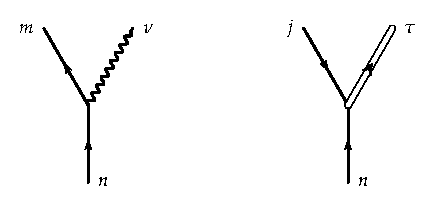
\includegraphics[width=0.65\textwidth]{pictures/9_7}
\par\end{centering}
\caption{\label{fig:9.7}单粒子耦合到单粒子加 ph 振动的相互作用顶点，以及单粒子耦合到单空穴加 pp 振动的相互作用顶点。}
\end{figure}

为了使讨论更加集中明晰，我们暂时忽略激发 pp 振动的可能性，即式 \ref{eq:9.134} 中的第二项自动掉落。在此物理假设下，式
\ref{eq:9.134} 中的加权因子 $1/3$ 相应地变为 $1/2$，即\footnote{我们在此处所使用的相互作用在形式上是原始的裸两体相互作用，正如迄今为止所有玻色展开理论一样。然而可以证明（参见附录 F），顶点（式
9.135）中的裸相互作用可以被不一定严格反对称的有效粒子-空穴相互作用所替代。}：
\begin{equation}
H_{\text{coupl}}=\frac{1}{2}\sum_{\nu}\left(\gamma^{\nu}_{mn}B^{\dagger}_{\nu}c^{\dagger}_{m}c_{n}+\text{h.c.}\right),\label{eq:9.135}
\end{equation}
其中 $\gamma^{\nu}_{kl}=\sum_{mi}C^{\nu*}_{m'i'}\bar{v}_{m'ki'l}$。

为了处理奇核的集体振动激发，我们形式上必须在多声子-单粒子基底（式 9.128）中对角化总 Hamiltonian（式 9.131）。在实际操作中，通常只需计及一个核心声子（如四极声子或八极声子）。偶偶核底层振子的非谐性越显著，在
Hamiltonian 的对角化中所需的多声子基底组态就越庞大。这一路线在 Alaga 及其合作者所发展的唯象模型中得到了长期的贯彻与应用
\cite{Al67,APS75}。正如我们在偶偶核中所看到的，玻色子描述对于转动核同样行之有效。因此，Hamiltonian（式
9.131）在原则上有能力系统描述当一个奇价粒子耦合到变形转子时所引发的所有微观物理效应，例如转动顺排（rotational alignment）或非轴对称三轴形变特征
\cite{AP76,PVD77}。然而在实际应用中，该 Hamiltonian 主要是针对近简谐振动核开展研究的，我们接下来就转向微扰论讨论。

\subsection{粒子-振动耦合（微扰论）\label{subsec:9.3.3_=007C92=005B50-=00632F=0052A8=008026=005408=00FF08=005FAE=006270=008BBA=00FF09}}

Hamiltonian（式 9.131）极适用于处理奇核中的集体振动。在最简单的情形下，我们将相邻的偶偶核视为纯简谐振子，此时体系的第一个集体激发态便是单粒子-振动声子耦合态。此外，在很多实际核中，粒子-振动耦合（PVC）非常微弱，使得
$H_{\text{coupl}}$ 完全可以在定态微扰论的框架下处理（即弱耦合情形）。

若我们要计算单粒子-振动状态由于耦合项所导致的能量位移，二阶微扰展开给出：
\begin{align}
\Delta E & =\Delta E_{1}+\Delta E_{2}\nonumber \\
 & =(p\mu|H_{\text{coupl}}|p\mu)+\sum_{\substack{kN\\
\ne p\mu
}
}\frac{(p\mu|H_{\text{coupl}}|kN)(kN|H_{\text{coupl}}|p\mu)}{E_{p\mu}-E_{kN}},\label{eq:9.136}
\end{align}
其中 $|p\mu)=\beta^{\dagger}_{p}B^{\dagger}_{\mu}|0)$ 代表未受微扰的单粒子加单声子组态，中间态
$|kN)$ 定义见式 \ref{eq:9.128}。在一阶微扰中，只有 $H_{\text{coupl}}$ 的第二项产生非零贡献，由式
\ref{eq:9.33}、\ref{eq:9.26} 与 \ref{eq:9.131} 可得：
\begin{align}
(p\mu|H_{\text{coupl}}|p\mu) & =-\frac{1}{2}\sum_{\nu}\left(V^{22}_{\mu\nu}\Gamma^{\mu p}_{\nu p}+\text{c.c.}\right)\nonumber \\
 & =-\frac{1}{4}\sum_{klq}\left(H^{22}_{klpq}C^{\mu*}_{kl}C^{\mu}_{pq}+\text{c.c.}\right).\label{eq:9.137}
\end{align}
在文献中，另一种与当前讨论密切相关的方法是 Bohr 与 Mottelson 提出的\textbf{核场论}（Nuclear Field
Theory, NFT）\cite{Mo67,BM75}，随后由 Broglia 等人进行了极其详尽的发展和系统应用 \cite{BBB77}。为了便于将本章表述与
NFT 进行精确比对，我们引入一条规则：每当 TDA 振幅（如式 9.137 中的 $C^{\mu}_{pq}$）的两个指标不汇合到同一个矩阵元且未被同时求和时，我们就必须利用
TDA 方程（式 8.10），从而使这类振幅变换为两个指标均作用在同一个 $\bar{v}$ 上并被闭合求和的形式。将此规则应用于一阶表达式（式
9.137）并在 HF 极限下将其严格局限于 ph 振动，我们得到：
\begin{equation}
\Delta E_{1}=-\sum_{i}\frac{|\gamma^{\mu}_{ip}|^{2}}{\Omega_{\mu}-\epsilon_{p}+\epsilon_{i}}.\label{eq:9.138}
\end{equation}
在二阶微扰中，只有 $H_{\text{coupl}}$ 的第一项做出贡献。它来源于包含零个玻色子（$N=0$）与两个玻色子（$N=2$）的中间态
$|kN)$。在 HF 极限下，该二阶项显式为\footnote{严格执行微扰论（式 9.136）对各项所给出的权重因子，与我们在此写出的形式略有不同（例如式 9.139 中的第一项原本会带有一个
$1/2$ 因子）。然而极为精妙的一点是：在对角化式 9.131 中的第二项时（即将其微扰级数求和至无穷阶），会产生与式 9.139
完全相同结构的额外修正项，将它们合并后恰好消去了 $1/2$ 因子。这一加权因子的微观来源在历史上曾引发了长期的争论 \cite{JDK69,El70}。简明准则是：在进行完全对角化时必须严格保留因子
$1/2$；而在仅执行最低阶微扰论时，该因子应当被吸收。}：
\begin{equation}
\Delta E_{2}=\sum_{n}\frac{|\gamma^{\mu}_{pn}|^{2}}{\Omega_{\mu}+\epsilon_{p}-\epsilon_{n}}+\sum_{n}\frac{|\gamma^{\mu}_{np}|^{2}}{\epsilon_{p}-\epsilon_{n}-\Omega_{\mu}}.\label{eq:9.139}
\end{equation}
根据图线规则，$\Delta E_{2}$ 的第一项和第二项分别对应于图 9.8 中的图 (a) 与图 (b)，而 $\Delta E_{1}$
则对应于图 (c)。图 9.8(d) 所示的微观过程显式涉及 $H^{40}$ 的两体矩阵元，如果我们一开始就在式 \ref{eq:9.131}
中保留 $H^{40}$ 并变换到 RPA 玻色子，就会自然导出该贡献。略去微小的 RPA 反向振幅，其解析表达式为：
\begin{equation}
\sum_{i}\frac{|\gamma^{\mu}_{pi}|^{2}}{\Omega_{\mu}+\epsilon_{p}-\epsilon_{i}}.\label{eq:9.140}
\end{equation}

\begin{figure}[H]
\begin{centering}
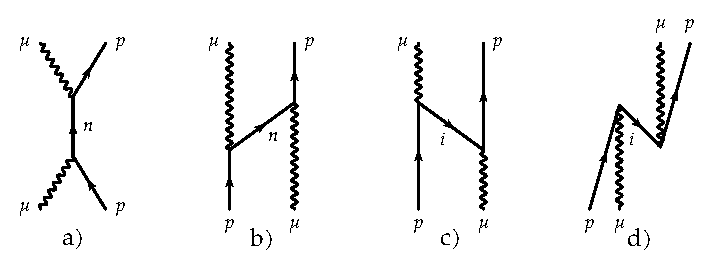
\includegraphics[width=0.75\textwidth]{pictures/9_8}
\par\end{centering}
\caption{\label{fig:9.8}代表单粒子-ph 振动耦合二阶能量贡献的四种可能微观图线。}
\end{figure}

图 9.8 中四种微观过程的物理图像极其清晰直观：
\begin{enumerate}
\item 图 (a)：集体振动声子与入射粒子融合成一个中间单粒子态，随后该中间态再次裂变发射出一个单粒子与一个集体振动声子；
\item 图 (b)：在粒子与集体振动共同传播的过程中，粒子自身虚拟激发一个声子并散射到另一个中间单粒子态上，随后该中间粒子吸收最初入射的振动声子；
\item 图 (c)：入射的集体振动声子虚拟解离为一个粒子-空穴对，其中的空穴随后与最初入射的价粒子复合湮灭，而剩余的激发粒子则重新退激构成出射的振动声子。这在本质上代表了空穴从一个粒子伙伴到另一个粒子的量子交换，因此确切体现了
Pauli 原理的禁戒修正。我们清楚地看到，该项正是源于 $H_{\text{coupl}}$ 中的高阶玻色子修正项；
\item 图 (d)：该过程在拓扑上与图 (a) 完全类似，唯一的关键区别在于中间传播的单粒子态被单空穴态所取代。正如前文所述，该过程直接源于多体系统基态中的两体量子关联。
\end{enumerate}
在文献中，Kisslinger 和 Sorensen \cite{KS63} 等人率先计入了图 (a) 与 (b) 的贡献；而空穴耦合同样具有决定性重要地位这一事实，则由
Hafele 首次明确指出 \cite{Ha67}。Mottelson 系统深入地评述了所有这些微观图线在 $^{209}\text{Bi}$
中单粒子与 $3^{-}$ 声子耦合中的相对重要性 \cite{Mo67}。

\subsection{粒子-振动耦合顶点的性质\label{subsec:9.3.4_=007C92=005B50-=00632F=0052A8=008026=005408=009876=0070B9=007684=006027=008D28}}

在继续深入讨论之前，我们首先详细探讨作为图 9.8 所示全部四个微观物理过程核心构件的耦合顶点 $\gamma^{\mu}_{kl}$（式
9.135）。为此，我们将该顶点变换到连续坐标空间 $\boldsymbol{r}$-表象中：
\begin{align}
\gamma^{\mu}_{kl} & =\int\mathrm{d}^{3}r_{1}\,\mathrm{d}^{3}r_{2}\,\phi_{k}(\boldsymbol{r}_{1})\gamma^{\mu}(\boldsymbol{r}_{1},\boldsymbol{r}_{2})\phi^{*}_{l}(\boldsymbol{r}_{2}),\label{eq:9.141}\\
\gamma^{\mu}(\boldsymbol{r}_{2},\boldsymbol{r}_{4}) & =\sum_{mi}\int\mathrm{d}^{3}r_{1}\,\mathrm{d}^{3}r_{3}\,\bar{v}(\boldsymbol{r}_{1},\boldsymbol{r}_{2},\boldsymbol{r}_{3},\boldsymbol{r}_{4})\phi^{*}_{m}(\boldsymbol{r}_{1})C^{\mu*}_{mi}\phi_{i}(\boldsymbol{r}_{3}).\nonumber 
\end{align}
为了进行定性阐明，我们近似将直接相互作用项视为纯 Wigner 类型的 $\delta$ 力（参见第 4 章）并忽略交换项，从而得到局域顶点形式：
\begin{equation}
\gamma^{\mu}(\boldsymbol{r}_{1},\boldsymbol{r}_{2})=\delta(\boldsymbol{r}_{1}-\boldsymbol{r}_{2})\gamma^{\mu}(\boldsymbol{r}_{1}),\qquad\gamma^{\mu}(\boldsymbol{r})\propto\delta\rho^{\mu}(\boldsymbol{r}),\label{eq:9.142}
\end{equation}
其中 $\delta\rho^{\mu}(\boldsymbol{r})$ 正是 8.3.1 节所详尽讨论的跃迁密度\footnote{在当前的定性讨论中，我们忽略了 RPA 与 TDA 激发振幅之间的细微差异。}。根据能量加权求和规则（参见
8.7.5 节）以及半经典流体模型考量 {[}参见 Tassie 模型，式 8.175{]}，跃迁密度可以用球对称基态密度 $\rho_{0}(r)$
的微商显式表达为：
\begin{equation}
\delta\rho^{\lambda}\propto\lambda r^{\lambda-1}Y_{\lambda0}\cdot\frac{\mathrm{d}\rho_{0}}{\mathrm{d}r}\qquad(\lambda\ne0).\label{eq:9.143}
\end{equation}
因此我们清楚地看到：粒子-振动耦合主要发生在原子核的核表面区域。

考察其与唯象液滴模型（参见 \cite{BM75} 以及第 1 章）之间的内在亲缘关系是极其富有启发的：正如在该模型中通常所假定的那样，对于固定的径向坐标
$r$，微小表面变形下的平均场核势阱 $V(\boldsymbol{r})$ 的等势面由式 1.7 给出 \cite{Ha74a}：
\begin{equation}
r_{\Omega}=r\left(1+\sum_{\lambda\mu}\alpha^{*}_{\lambda\mu}Y_{\lambda\mu}(\Omega)\right).\label{eq:9.144}
\end{equation}
这精确等价于等势面方程：
\begin{equation}
V(r_{\Omega},\Omega)=V_{0}(r),\label{eq:9.145}
\end{equation}
其中 $V_{0}(r)$ 是未形变的球对称中心势。因此对于任意实际坐标 $r_{\Omega}$，我们只需通过坐标尺度缩放即可表示实际势阱：
\begin{equation}
V(r_{\Omega},\Omega)=V_{0}\left[\frac{r_{\Omega}}{1+\sum_{\lambda\mu}\alpha^{*}_{\lambda\mu}Y_{\lambda\mu}(\Omega)}\right].\label{eq:9.146}
\end{equation}
对于微小的表面振动变形，我们展开至形变参数 $\alpha_{\lambda\mu}$ 的一阶（将 $r_{\Omega}$ 记回
$r$）：
\begin{equation}
V(r,\Omega)=V_{0}(r)-r\frac{\mathrm{d}V_{0}(r)}{\mathrm{d}r}\sum_{\lambda\mu}\alpha^{*}_{\lambda\mu}Y_{\lambda\mu}(\Omega)+O(\alpha^{2}).\label{eq:9.147}
\end{equation}
因此，粒子与核表面形变之间的耦合作用项具有如下标准形式：
\begin{equation}
H_{\text{coupl}}=-k(r)\sum_{\lambda\mu}\alpha^{*}_{\lambda\mu}Y_{\lambda\mu}(\Omega),\label{eq:9.148}
\end{equation}
其形状因子为：
\begin{equation}
k(r)=r\frac{\mathrm{d}V_{0}}{\mathrm{d}r}.\label{eq:9.149}
\end{equation}
按照液滴模型的处方对表面振动模式进行二次量子化（第 1 章），我们就精确重现了与微观 $H_{\text{coupl}}$（式 9.135）完全一致的算符形式。在核势阱大体跟随核子密度的合理假定下，Tassie
模型（参见 13.3.3 节）与液滴模型对四极模式给出了形式完全相同的形状因子 $k(r)$（仅差一个常数因子），而在高阶多极模式下两者的径向幂次略有不同。多年来，这类唯象粒子-振动耦合顶点被极其广泛地应用于描述单核子与核芯
$2^{+}$ 或 $3^{-}$ 表面振动的耦合问题中（参见 Arima 和 Hamamoto 的权威综述 \cite{AH71b}、Hamamoto
的综述 \cite{Ha74a} 及其所引文献，以及 Alaga、Paar 和 Sips 编辑的振动核国际专题会议文集 \cite{APS75}）。

\section{\label{sec:9.3.5}有效电荷}

在本节中，我们将玻色展开方法应用于奇核系统，以深入研究所谓的“有效电荷”（effective charge）概念。为此，我们从 Hamiltonian
式 (\ref{eq:9.131}) 与式 (\ref{eq:9.135}) 出发，通过向 RPA 玻色子作正则变换（在微扰展开的最低阶上这一步并不困难），可以得到如下表达式：

\begin{equation}
H=E_{\text{RPA}}+\sum_{k}\epsilon_{k}c^{\dagger}_{k}c_{k}+\sum_{\mu}\Omega_{\mu}O^{\dagger}_{\mu}O_{\mu}+\sum_{\mu kl}\left(\gamma^{\mu}_{kl}O^{\dagger}_{\mu}c^{\dagger}_{k}c_{l}+\text{h.c.}\right),\label{eq:9.150}
\end{equation}
其中微观粒子-振动耦合顶点为：
\begin{equation}
\gamma^{\mu}_{kl}=\sum_{mi}\left(X^{\mu}_{mi}\bar{v}_{mkil}+Y^{\mu}_{mi}\bar{v}_{ikml}\right).\label{eq:9.151}
\end{equation}
（此处我们略去了 $\frac{1}{2}$ 因子，因为我们将应用最低阶微扰论；参见第 386 页脚注的讨论）。在有一阶微扰论中，奇核系统的本征波函数可表示为：
\begin{equation}
|\tilde{k})=c^{\dagger}_{k}|0)+\sum_{\mu l}\frac{\gamma^{\mu}_{lk}}{\epsilon_{k}-\epsilon_{l}-\Omega_{\mu}}O^{\dagger}_{\mu}c^{\dagger}_{l}|0).\label{eq:9.152}
\end{equation}
我们感兴趣的是这种“粒子-声子”修正对于电磁多极算符 $T$ 的矩阵元所带来的贡献。为此，我们首先必须利用式 (E.11) 将 $T$
变换到玻色表象式 (\ref{eq:9.130}) 中：
\begin{equation}
T=T^{0}+\sum_{mn}T_{mn}c^{\dagger}_{m}c_{n}-\sum_{ij}T_{ij}c_{j}c^{\dagger}_{i}+\sum_{mi}\left(T_{mi}c^{\dagger}_{m}c_{i}+\text{h.c.}\right),\label{eq:9.153}
\end{equation}
在一阶近似下，我们得到\footnote{在下文中，我们假定偶核核芯的基态期望值 $T^{0}$ 恒等于零。}：
\begin{equation}
T_{B}=\sum_{mn}T_{mn}c^{\dagger}_{m}c_{n}-\sum_{ij}T_{ij}c_{j}c^{\dagger}_{i}+\sum_{\mu}\left(T^{\mu}O^{\dagger}_{\mu}+\text{h.c.}\right),\label{eq:9.154}
\end{equation}
其中声子跃迁矩阵元为：
\begin{equation}
T^{\mu}=\sum_{mi}\left(T_{mi}X^{\mu*}_{mi}+T_{im}Y^{\mu*}_{mi}\right).\label{eq:9.155}
\end{equation}
现在我们可以计算有效矩阵元，其定义为：
\begin{align}
T^{\text{eff}}_{kl} & =(\tilde{k}|T_{B}|\tilde{l})\nonumber \\
 & =T_{kl}+\sum_{\mu}\left(\frac{\gamma^{\mu}_{kl}T^{\mu*}}{\epsilon_{l}-\epsilon_{k}-\Omega_{\mu}}+\frac{\gamma^{\mu*}_{lk}T^{\mu}}{\epsilon_{k}-\epsilon_{l}-\Omega_{\mu}}\right).\label{eq:9.156}
\end{align}

\begin{figure}[H]
\begin{centering}
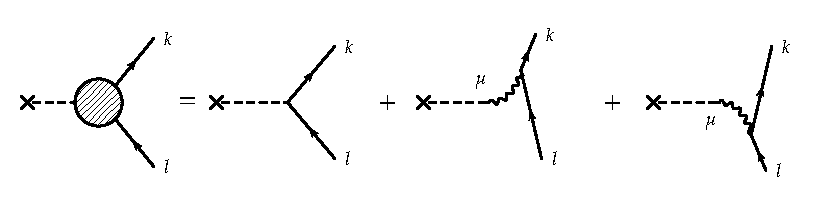
\includegraphics[width=0.7\textwidth]{pictures/9_9}
\par\end{centering}
\caption{\label{fig:9.9}有效电荷的费曼图图形表示。外场激发了核芯的虚振动声子，进而与外加价核子发生相互作用。}
\end{figure}

由式 (\ref{eq:9.156}) 可以看出，粒子-振动耦合将裸矩阵元 $T_{kl}$ 重整化为有效矩阵元 $T^{\text{eff}}_{kl}$。其微观物理根源在于：外场可以激发偶核核芯的虚振动（声子激发），并通过核力与外部价核子发生强烈的动力学相互作用。若该振动模式具有高度的集体性，它将使得矩阵元数值发生极为显著的改变。有效矩阵元的微观机制在\ref{fig:9.9}中给出了直观的费曼图表示。

体现这一动力学过程重要性的典型范例是闭壳核邻近单粒子态的有效电荷。在 2.7.2 节中我们已经看到，为了复现实验测得的质子与中子电多极矩和跃迁几率，必须引入有效电荷（通常取
$e^{\text{eff}}_{\text{p}}\approx2$，$e^{\text{eff}}_{\text{n}}\approx1$）。其物理原因正是\ref{fig:9.9}所示的核芯虚声子激发极化效应。我们的有效矩阵元式
(\ref{eq:9.156}) 可以进一步改写为：
\begin{equation}
T^{\text{eff}}_{kl}=T_{kl}+\sum_{mn}e^{\text{pol}}_{klmn}T_{mn},\label{eq:9.157}
\end{equation}
其中极化电荷 $e^{\text{pol}}=e^{\text{pol}}(\epsilon_{k}-\epsilon_{l})$
此时是一个依赖于单粒子能量差 $\epsilon_{k}-\epsilon_{l}$ 的动力学算符。将这一动力学算符用一个常数替代，便对应于唯象的有效电荷概念：
\begin{equation}
e^{\text{eff}}=1+e^{\text{pol}}.\label{eq:9.158}
\end{equation}
例如，在计算四极矩的有效电荷时，我们必须对偶核核芯的所有集体 $2^{+}$ 态的贡献进行求和。特别地，这意味着必须将巨四极共振（GQR，参见第
8 章）的激发全面计入。这类微观计算已在例如 Pb 同位素区开展 \cite{RBS73}，所得理论预言与实验结果高度符合。

有效矩阵元的定量计算需要预先求解 RPA 振幅 $X^{\mu}_{mi}$、$Y^{\mu}_{mi}$ 及其本征能量 $\Omega_{\mu}$。利用
RPA 方程（式 8.131），我们可以直接推导出关于 $T^{\text{eff}}$ 的闭合积分方程（亦可参见 Migdal
的工作 \cite{Mi67}）：
\begin{equation}
T^{\text{eff}}_{kl}(\omega)=T_{kl}+\sum_{pq}\bar{v}_{kqlp}\frac{n_{q}-n_{p}}{\omega-\epsilon_{p}+\epsilon_{q}}T^{\text{eff}}_{pq}(\omega).\label{eq:9.159}
\end{equation}
该方程直观地揭示了介质中的粒子-空穴极化传播子如何将外场有效驱动力重整化。

\section{\label{sec:9.3.6}\label{subsec:9.3.6_=004E2D=007B49=008026=005408=004E0EDyson=0073BB=008272=005C55=005F00}中间耦合与
Dyson 玻色展开}

前述各节中所阐述的粒子-振动耦合微扰处理方案，显然只有在极端弱耦合极限下才是严格有效的；在该极限下，$H_{\text{coupl}}$
的非对角矩阵元相比于对角能量项必须极其微小。然而事实表明，即便在被视作弱耦合原型的典型范例——$^{209}\text{Bi}$
的七重态（septuplet，详见下文讨论）中，这一条件也未能完全得到满足。为了克服微扰论的局限性，我们固然可以在未微扰基底（$H_{\text{coupl}}=0$）中对全
Hamiltonian 式 (\ref{eq:9.130}) 与式 (\ref{eq:9.131}) 进行严格对角化，但与此同时，我们必须将
Hamiltonian 的玻色展开式 (\ref{eq:9.131}) 推进到更高阶次，以确保达到所谓的水平收敛（horizontal
convergence，参见\ref{fig:9.3}）。然而迄今为止，这一完整方案在实践中极少被完全实现，主要应用于奇核系统的实际理论往往是另一类玻色理论——核场论（Nuclear
Field Theory, NFT；例如参见 \cite{Re75b,BBB77} 及其所引文献）。NFT 是一种高度非线性的代数理论，但已有严格证明表明
\cite{IRS79}，存在一种精巧的数学对应关系，可将非线性的 NFT 精确归结为线性的 Dyson 玻色展开（DBE），而
DBE 理论本身也已被成功应用于处理许多真实的复杂原子核系统 \cite{DJ73,RS74b,SWR76,IRS80}。鉴于线性代数方程在计算与概念处理上通常远比非线性理论简便，我们在本节中将专门阐述
DBE 方法。这使得我们能够大范围沿用在偶核系统中所建立的形式体系。正如偶核情形一样，奇核系统的 DBE 展开同样具有严格截断的有限阶代数结构。

对于集体玻色子，费米子对算符在奇核系统中的 DBE 映射形式为（非集体版本可参见 \cite{DJ73}）：
\begin{align}
(b^{\dagger}_{\mu})_{B} & =B^{\dagger}_{\mu}-\frac{1}{2}\sum_{\nu\rho\sigma}\Gamma^{\nu\rho}_{\mu\sigma}B^{\dagger}_{\nu}B^{\dagger}_{\rho}B_{\sigma}-\sum_{kl\nu}\Gamma^{\nu k}_{\mu l}B^{\dagger}_{\nu}\beta^{\dagger}_{k}\beta_{l},\nonumber \\
(b_{\mu})_{B} & =B_{\mu},\label{eq:9.160}\\
(a_{\mu\nu})_{B} & =\sum_{\rho\sigma}\Gamma^{\mu\rho}_{\nu\sigma}B^{\dagger}_{\rho}B_{\sigma}+\sum_{kl}\Gamma^{\mu k}_{\nu l}\beta^{\dagger}_{k}\beta_{l}.\nonumber 
\end{align}
将这些代数映射代入准粒子 Hamiltonian 式 (\ref{eq:9.32}) 中，并在如下由单准粒子与单声子构成的截断基底空间中进行对角化：
\begin{equation}
|A+1,\nu)=\sum_{p}C^{(\nu)}_{p}\beta^{\dagger}_{p}|0)+\sum_{p\mu}C^{(\nu)}_{p\mu}\beta^{\dagger}_{p}B^{\dagger}_{\mu}|0),\label{eq:9.161}
\end{equation}
即可直接导出如下久期矩阵方程：
\begin{equation}
\sum_{p'\mu'}\begin{pmatrix}\delta_{pp'}E_{p} & \frac{1}{2}\gamma^{\mu'*}_{p'p}\\
\frac{1}{2}\gamma^{\mu}_{pp'} & (\Omega_{\mu}+E_{p})\delta_{pp'}\delta_{\mu\mu'}+B_{p\mu p'\mu'}
\end{pmatrix}\begin{pmatrix}C^{(\nu)}_{p'}\\
C^{(\nu)}_{p'\mu'}
\end{pmatrix}=\omega^{(\nu)}\begin{pmatrix}C^{(\nu)}_{p}\\
C^{(\nu)}_{p\mu}
\end{pmatrix},\label{eq:9.162}
\end{equation}
其中 $\gamma^{\mu}_{p'p}$ 定义于式 (\ref{eq:9.132})，而诱导对角修正矩阵 $B$ 具有显式结构：
\begin{equation}
B_{p\mu p'\mu'}=-\sum_{l}(\Omega_{\mu'}-E_{l}-E_{p})C^{\mu}_{p'l}C^{\mu'*}_{pl}.\label{eq:9.163}
\end{equation}
在建立式 (\ref{eq:9.162}) 时，我们利用了准粒子 TDA 方程 {[}式 (8.10) 与式 (9.70){]}。矩阵元
(\ref{eq:9.162}) 的求值十分直接，仅有对 $H^{11}$ {[}见式 (9.32){]} 的处理较为繁琐。在无配对关联的极限下，对
$\mu'$ 的求和自然同时涵盖了 $ph$ 与 $pp$ 振动模式。这一代数对应关系可借助式 (9.133)、(8.201)
与 (8.202) 轻松推导。显而易见，与偶核情形完全相同，式 (\ref{eq:9.162}) 中的本征矩阵是非厄米的。

为了深入剖析修正矩阵 $B$ 的微观物理涵义，我们转到无超流关联的 HF 极限，在此极限下可以明确区分 $ph$ 与 $pp$
振动激发。此时我们清晰地看到，矩阵 $B$ 不仅能够耦合 $p\text{-}ph$ 与 $h\text{-}pp$ 组态，还同时在
$p\text{-}ph$ 组态彼此之间产生耦合。对照\ref{fig:9.8}(c) 所示的自能交换图，后一种耦合精确执行了对
Pauli 原理的动力学修正。由于显而易见的原因，$h\text{-}pp$ 与 $h\text{-}pp$ 组态之间不存在 Pauli
原理的重叠干涉，因此相应的矩阵元 $B_{h\text{-}pp,h\text{-}pp}$ 自然恒等于零。展开系数 $C^{(\nu)}_{p\mu}$
的物理涵义非常明确：它作为谱因子（spectroscopic factor），刻画了集体激发态在多大程度上由奇核准粒子的非关联运动与偶核核芯的集体声子振动耦合而成。这里的准粒子既可以是价粒子，也可以是空穴。例如，$^{209}\text{Bi}$
七重态的本征系数 $C^{(\nu)}_{p\mu}$ 直观揭示了该态究竟有多少成分是由单粒子与 $^{208}\text{Pb}$
的 $ph$ 振动耦合而成，又有多少成分是由空穴与 $^{210}\text{Pb}$、$^{210}\text{Po}$ 及
$^{210}\text{Bi}$ 的 $pp$ 振动耦合而成。必须指出的是，式 (\ref{eq:9.162}) 对应于一个非正交基底空间，因此这些系数仅代表相对几率幅。

矩阵方程 (\ref{eq:9.162}) 的代数维度显然远大于原始费米子物理空间的维度；但由于玻色子具有极强的集体性，我们完全有理由对基底空间进行大幅度截断。由于基底的过完备性，式
(\ref{eq:9.162}) 的解集不可避免地混杂着非物理的赝态（spurious solutions）。然而与偶核情形完全类似
{[}参见式 (9.98){]}，这些赝态全部落在自由三准粒子未微扰能量的极高位置处，因而远高于我们所关心的低能集体振动能级。因此，对于基底截断已经实现垂直收敛（vertical
convergence，见\ref{fig:9.3}）的系统，赝态绝不会造成任何实际困扰。在此情形下，所有感兴趣的低能本征值均为严格实数，矩阵的非厄米性亦不构成障碍。而对于核芯集体性并不十分显著、赝态与物理态可能相互交织的情形，一种极佳的处方是对范数度规矩阵进行对角化，通过剔除其零本征值（或实际计算中小于某一阈值
$\epsilon$ 的小本征值），将方程 (\ref{eq:9.162}) 严格变换为一个正交归一的厄米本征问题 \cite{IRS80,BSL79}。通过对剩余的对角范数矩阵求平方根并求逆，即可完成基底的正交归一化。该过程的具体数学细节将在
10.2 节中深入阐述。厄米化后的问题维度绝不会超过原始费米子空间的真实维度，从而彻底在数学上排除了任何赝态的侵入。正交归一化基底在精确计算电磁跃迁几率时亦展现出突出的代数优势。

为了深入领会上述物理与代数机制，考察一个虽然带有学术假定但完全可严格解析求解的三粒子模型是极具启发性的：在忽略配对关联且在闭壳核外存在三个价核子的情形下，式
(\ref{eq:9.162}) 中的粒子-振动耦合顶点 $\gamma$ 严格为零，我们得到如下简化的本征矩阵方程（其中 $p,m,n$
代表单粒子态，$\tau,\tau'$ 代表 $pp$ 振动模式）：
\begin{equation}
\sum_{\tau'p'}B_{p\tau p'\tau'}C^{(\nu)}_{p'\tau'}=\left(\omega^{(\nu)}-\Omega_{\tau}-\epsilon_{p}\right)C^{(\nu)}_{p\tau},\label{eq:9.164}
\end{equation}
其中相互作用核为：
\begin{equation}
B_{p\tau p'\tau'}=\sum_{n}C^{\tau*}_{p'n}(\Omega_{\tau'}-\epsilon_{n}-\epsilon_{p})C^{\tau'}_{np},\label{eq:9.165}
\end{equation}
这里的 $C^{\tau}_{mn}$ 与 $\Omega_{\tau}$ 是标准 $pp$-TDA 方程的本征解。

\begin{figure}[H]
\begin{centering}
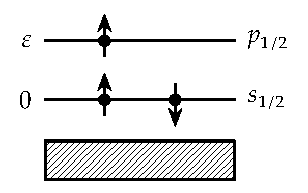
\includegraphics[width=0.4\textwidth]{pictures/9_10}
\par\end{centering}
\caption{\label{fig:9.10}解析可解模型的三个价核子能级组态示意图。}
\end{figure}

作为具体模型，我们考虑处于 $s_{1/2}$ 与 $p_{1/2}$ 能级中的三个价核子系统（如\ref{fig:9.10}所示）。在全部组态中，具有负宇称且自旋向上的物理纯费米子态仅有一个：
\[
|\alpha\rangle=a^{\dagger}_{s\frac{1}{2}}a^{\dagger}_{s-\frac{1}{2}}a^{\dagger}_{p\frac{1}{2}}|D\rangle.
\]
该纯物理态相对于核芯 $|D\rangle$ 的能量期望值可以直接计算求得：
\begin{align*}
\langle\alpha|H|\alpha\rangle-\langle D|H|D\rangle & =\epsilon+v_{s\frac{1}{2}s-\frac{1}{2},s\frac{1}{2}s-\frac{1}{2}}+v_{s\frac{1}{2}p\frac{1}{2},s\frac{1}{2}p\frac{1}{2}}+v_{s-\frac{1}{2}p\frac{1}{2},s-\frac{1}{2}p\frac{1}{2}}\\
 & =\epsilon+G+F+H.
\end{align*}
接下来我们需要计算两体激发态；假定双粒子剩余相互作用仅有对角矩阵元非零，我们可解出如下五个相关的两体 $\tau$ 模式：
\begin{align*}
C^{\tau_{1}}_{s\frac{1}{2}p\frac{1}{2}} & =1,\quad\Omega_{\tau_{1}}=\epsilon+F;\\
C^{\tau_{2}}_{s-\frac{1}{2}p\frac{1}{2}} & =1,\quad\Omega_{\tau_{2}}=\epsilon+H;\\
C^{\tau_{3}}_{s\frac{1}{2}s-\frac{1}{2}} & =1,\quad\Omega_{\tau_{3}}=G;\\
C^{\tau_{4}}_{s\frac{1}{2}p-\frac{1}{2}} & =1,\quad\Omega_{\tau_{4}}=\epsilon+v_{s\frac{1}{2}p-\frac{1}{2},s\frac{1}{2}p-\frac{1}{2}}:=\epsilon+I;\\
C^{\tau_{5}}_{p\frac{1}{2}p-\frac{1}{2}} & =1,\quad\Omega_{\tau_{5}}=2\epsilon+v_{p\frac{1}{2}p-\frac{1}{2},p\frac{1}{2}p-\frac{1}{2}}:=2\epsilon+J.
\end{align*}
对应的五种粒子-玻色子 $p\tau$ 组态展示于\ref{fig:9.11}中。

\begin{figure}[H]
\begin{centering}
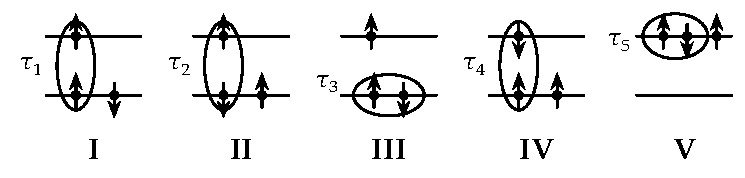
\includegraphics[width=0.7\textwidth]{pictures/9_11}
\par\end{centering}
\caption{\label{fig:9.11}三粒子模型中的五种可能的粒子-玻色子组态示意图（标号分别为 I、II、III、IV、V）。}
\end{figure}

由\ref{fig:9.11}可以极其清晰地看到：由于在构造基底态时忽略了 Pauli 原理，基底维度从物理上的 1 维急剧膨胀为
5 维，即此时的玻色空间是严重过完备的。现在我们来具体计算式 (\ref{eq:9.165}) 的相互作用矩阵（将不同的 $p\tau$
组态简记为 I、II、III、IV、V）：
\begin{align*}
B_{\text{I I}} & =\sum_{n}C^{\tau_{1}}_{s-\frac{1}{2}n}(\epsilon+F-\epsilon_{n}-0)C^{\tau_{1}}_{ns-\frac{1}{2}}=0,\\
B_{\text{I II}} & =\sum_{n}C^{\tau_{1}}_{s-\frac{1}{2}n}(\epsilon+H-\epsilon_{n}-0)C^{\tau_{2}}_{ns-\frac{1}{2}}=-H,\\
B_{\text{I III}} & =-G,\\
B_{\text{I IV}} & =B_{\text{I V}}=0.
\end{align*}
对全矩阵的全部元素依此类推，我们最终得到本征方程 (\ref{eq:9.164}) 的如下久期行列式：
\[
\begin{vmatrix}\epsilon+F-\omega^{(\alpha)} & -H & -G & 0 & 0\\
-F & \epsilon+H-\omega^{(\alpha)} & G & 0 & 0\\
-F & H & \epsilon+G-\omega^{(\alpha)} & 0 & 0\\
0 & 0 & 0 & \epsilon-\omega^{(\alpha)} & 0\\
0 & 0 & 0 & 0 & 2\epsilon-\omega^{(\alpha)}
\end{vmatrix}=0.
\]
显而易见，该矩阵是非厄米的。直接求出行列式的特征多项式根，可得到其全部本征值为：
\[
\omega^{(1)}=\omega^{(2)}=\omega^{(3)}=\epsilon;\quad\omega^{(4)}=2\epsilon;\quad\omega^{(5)}=\epsilon+F+G+H.
\]
我们由此惊奇而漂亮地发现：本征谱精确地重现了真物理态的能量 $\epsilon+F+G+H$，而伴随产生的四个多余本征态全部是不具相互作用的未微扰纯单粒子（或空穴）能量！这与我们在偶核
DBE 理论中推得的结论完全契合：过完备基底引入的全部非物理赝态严格定域于未微扰单粒子能量处。尽管本模型具有教学演示的理想简化性质，但在偶核核芯存在极强集体激发态的实际原子核中，通过截断后所需对角化的有效玻色矩阵规模将远远小于全费米子多体组态空间。

\begin{figure}[H]
\begin{centering}
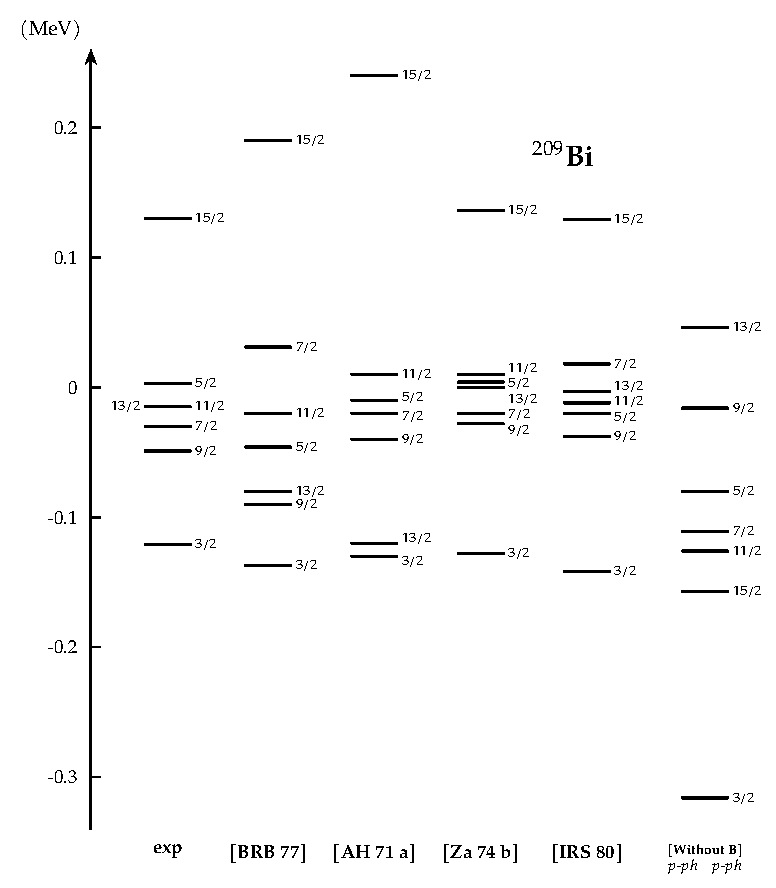
\includegraphics[width=0.75\textwidth]{pictures/9_12}
\par\end{centering}
\caption{\label{fig:9.12}$^{209}\text{Bi}$ 中粒子-振动耦合态（七重态）的能谱：展示了实验测量能级以及不同理论作者给出的计算结果。在最后一列中，人为略去了式
(9.162) 中的 $B_{p\text{-}ph,p\text{-}ph}$ 矩阵元，以直观彰显 Pauli 原理的剧烈重整化效应。零能量基准线取为
$^{208}\text{Pb}$ 中 $3^{-}$ 态的激发能（2.614 MeV）。}
\end{figure}

作为具体物理应用，\ref{fig:9.12}展示了利用 DBE 求解式 (\ref{eq:9.162}) 并逐步扩展基底维度直至垂直收敛所计算的
$^{209}\text{Bi}$ 七重态（septuplet）能谱。图中同时列出了利用核场论（NFT）\cite{BBB77}
以及其他学者采用不同微观方法 \cite{AH71a,Za74b} 所得的理论结果与实验数据的系统比对。在\ref{tab:9.2}中，我们给出了若干主要波函数分量
$C^{(\nu)}_{p\mu}$（谱因子），以清晰展示其相对重要性。\ref{fig:9.12}无可辩驳地证明了严谨计入 Pauli
原理修正的关键性：若人为关闭式 (\ref{eq:9.162}) 中的 $B_{p\text{-}ph,p\text{-}ph}$
矩阵元（即图中最右侧一列），计算出的能级裂距将产生完全背离实验的严重畸变。理论与实验之间尚存的微小偏差主要归因于两点：第一，$2p\text{-}1h$
组态是构筑七重态的主导成分，计算中处理了其与 $1p$ 空间的弱耦合，但忽略了与 $3p\text{-}2h$ 复杂组态的耦合；出于对称性考虑，高阶组态理应被完整计入，然而这在数值计算实践中极其繁复；第二，基底截断和相互作用参数的选取仍存在微小唯象调整空间。

\begin{table}[H]
\caption{\label{tab:9.2}$^{209}\text{Bi}$ 七重态中若干粒子-振动耦合态的波函数结构（以谱因子 $C_{p\mu}$
给出）。主导成分 $\pi h_{9/2}\otimes{}^{208}\text{Pb}(3^{-})$ 归一化为 1.0（引自
\cite{IRS80}）。}

\centering{}%
\begin{tabular}{lccc}
\toprule 
$p\quad\mu$ & $3/2$ & $5/2$ & $7/2$\tabularnewline
\midrule
纯单粒子态 & 0.005 & 0.001 & 0.026\tabularnewline
$\pi h_{9/2}\otimes{}^{208}\text{Pb}(3^{-})$ & 1.0 & 1.0 & 1.0\tabularnewline
$\pi h_{9/2}\otimes{}^{208}\text{Pb}(6^{+}_{1})$ & $-0.385$ & 0.266 & $-0.233$\tabularnewline
$\nu g_{9/2}\otimes{}^{208}\text{Bi}(6^{+}_{2})$ & $-0.406$ & 0.356 & $-0.320$\tabularnewline
$\nu i_{11/2}\otimes{}^{208}\text{Bi}(6^{+}_{1})$ & 0.100 & $-0.155$ & 0.211\tabularnewline
$\nu i_{11/2}\otimes{}^{208}\text{Bi}(7^{+}_{1})$ & $-0.318$ & 0.282 & $-0.232$\tabularnewline
$(\pi d_{3/2})^{-1}\otimes{}^{210}\text{Po}(0^{+})$ & 0.326 & — & —\tabularnewline
$(\pi d_{3/2})^{-1}\otimes{}^{210}\text{Po}(2^{+})$ & 0.233 & 0.231 & 0.095\tabularnewline
$(\pi d_{3/2})^{-1}\otimes{}^{210}\text{Po}(4^{+})$ & — & 0.200 & 0.282\tabularnewline
$(\nu p_{3/2})^{-1}\otimes{}^{210}\text{Bi}(1^{-})$ & 0.286 & $-0.128$ & —\tabularnewline
$(\nu p_{3/2})^{-1}\otimes{}^{210}\text{Bi}(2^{-})$ & 0.225 & 0.205 & 0.090\tabularnewline
$(\nu p_{3/2})^{-1}\otimes{}^{210}\text{Bi}(3^{-})$ & 0.151 & 0.234 & 0.191\tabularnewline
$(\nu p_{3/2})^{-1}\otimes{}^{210}\text{Bi}(4^{-})$ & — & $-0.181$ & $-0.255$\tabularnewline
$(\nu p_{3/2})^{-1}\otimes{}^{210}\text{Bi}(5^{-})$ & — & — & $-0.235$\tabularnewline
\bottomrule
\end{tabular}
\end{table}


\section{\label{sec:9.3.7}其它粒子-振动耦合计算}

正如我们在本节伊始所指出的，在核物理中存在许多不同类型的弱耦合理论应用，我们在此无法一一详尽展开。例如，对于必须计入超流对关联的球形开壳核系统，我们尚未讨论各类准粒子-声子耦合理论
\cite{KS63,DJ73}。在这一方向上最为精深且先进的微观理论之一——虽然其庞大的代数体系已经超出了本书的范围——是由 Marumori
及其合作者所创立的理论体系 \cite{KMM72,KMM75a,KMM75b}。

\begin{figure}[H]
\begin{centering}
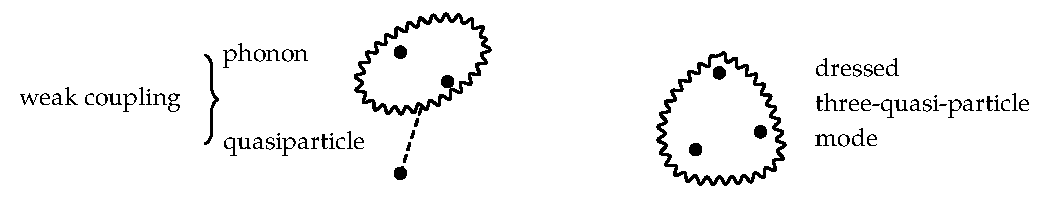
\includegraphics[width=0.7\textwidth]{pictures/9_13}
\par\end{centering}
\caption{\label{fig:9.13}准粒子-声子（弱耦合）与缀饰三准粒子模式（强耦合）的示意图表示。}
\end{figure}

该理论不仅能够描述弱耦合情形，而且能够极其精确地刻画三个准粒子发生强烈纠缠与多体重整化的强耦合情形（缀饰三准粒子模式，dressed
three-quasiparticle mode，见\ref{fig:9.13}；当然 DBE 同样具备这种能力）；更重要的是，它系统计入了基态关联（ground
state correlations），并且严格排除了由于 BCS 理论破坏粒子数守恒所引入的非物理赝成分。

\begin{figure}[H]
\begin{centering}
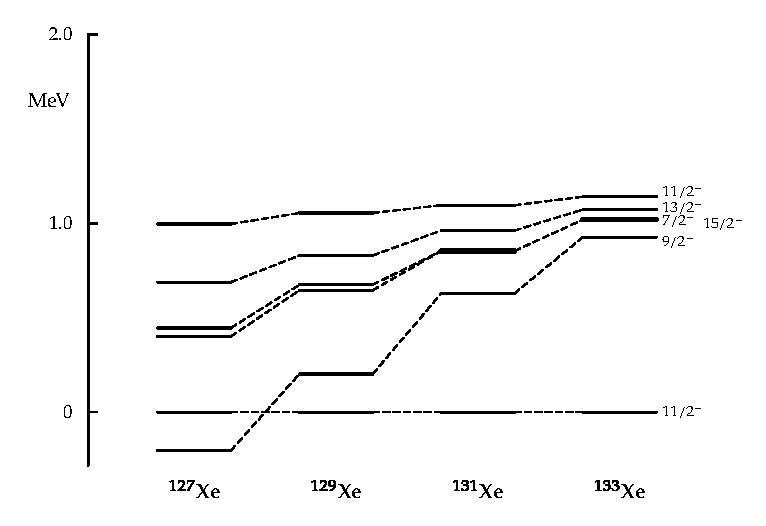
\includegraphics[width=0.7\textwidth]{pictures/9_14}
\par\end{centering}
\caption{\label{fig:9.14}一系列 Xe 同位素中粒子-振动耦合态的能量系统学演化（引自 \cite{KMM75a}）。}
\end{figure}

展现该理论威力的一个极佳应用范例，是一系列 Xe 与 Te 同位素中奇中子 $h_{11/2}$ 态与核芯 $2^{+}$ 声子态的耦合问题，其展现了从弱耦合向强耦合平滑过渡的清晰物理图像（见\ref{fig:9.14}）。在
Xe 同位素链中，从 $^{133}\text{Xe}$ 走向 $^{127}\text{Xe}$——亦即朝向 $h_{11/2}$
壳层中央演化时，我们观察到多重态的能级劈裂急剧增大；对于 $^{127}\text{Xe}$，能级劈裂已经如此剧烈，以至于多重态中能量最低的分支——即
$9/2^{-}$ 态（强烈关联的缀饰三准粒子态）——其能量甚至反常地低于奇中子本身的未微扰单粒子 $11/2^{-}$ 态！这类能级在核物理中通常被称为“反常耦合态”（abnormal
coupling states）。其物理起源归结为两种协同效应：
\begin{enumerate}
\item 几何代数效应：在单粒子角动量 $j$ 与 $2^{+}$ 声子的角动量耦合中，$j-1$ 态在几何对称性上始终是该多重态中能量最低的成员（参见
\cite{KMM75a}）；
\item 动力学关联效应：随着原子核越来越接近壳层中部，基态（BCS）配对关联急剧增强。可以严格证明，此时\ref{fig:9.8}(c)
所代表的对易自能修正图变得极其巨大且占据主导地位。
\end{enumerate}
在 Te 同位素链中，这种耦合强度相对较弱，因而在实验上并未发生反常耦合反转现象。理论所给出的能级系统学演化趋势与实验测量得到了非常完美的符合。

\section{\label{sec:9.3.8}偶偶系统中的弱耦合}

在原子核理论中，还广泛存在着许多其他类型的弱耦合物理图像。弱耦合决非仅仅局限于奇 $A$ 核系统——在偶偶核中同样存在显著的弱耦合现象。例如，$^{208}\text{Pb}$
中的双 $3^{-}$ 声子四重态（$3^{-}\otimes3^{-}\to0^{+},2^{+},4^{+},6^{+}$；迄今实验上仅确证了
$0^{+}$ 与 $2^{+}$ 两个能级）极有可能属于典型的弱耦合类型 \cite{BBN74a,Sch76}。从理论观点来看，最好能采用一种能够同时统一描述弱耦合、中间耦合乃至强耦合情境的理论形式体系；正如前文所展示的，对于双幻核或邻近幻核的体系，Dyson
玻色展开（DBE）正是这样一种理想的微观形式体系。

在处理单声子与双声子态的动力学耦合时，偶核系统的波函数可表达为如下形式：
\begin{equation}
|\tilde{\nu})=\sum_{\mu}C^{(\nu)}_{\mu}\tilde{B}^{\dagger}_{\mu}|0)+\sum_{\mu_{1}\mu_{2}}C^{(\nu)}_{\mu_{1}\mu_{2}}\tilde{B}^{\dagger}_{\mu_{1}}\tilde{B}^{\dagger}_{\mu_{2}}|0),\label{eq:9.166}
\end{equation}
其中指标 $\mu$ 的求和自然同时包括 $ph$ 与 $pp$ 振动模式。相应的 DBE 矩阵具有如下结构：
\begin{equation}
\begin{pmatrix}\Omega_{\mu}\delta_{\mu\mu'} & -\frac{1}{2}\sum_{kl}\gamma^{\mu_{1}'}_{kl}\Gamma^{\mu_{2}'k}_{\mu'l}-(\mu_{1}'\leftrightarrow\mu_{2}')\\
-\frac{1}{2}\sum_{kl}\gamma^{\mu_{1}}_{kl}\Gamma^{\mu_{2}k}_{\mu'l}-(\mu_{1}\leftrightarrow\mu_{2}) & (\Omega_{\mu_{1}}+\Omega_{\mu_{2}})\delta_{\mu_{1}\mu_{1}'}\delta_{\mu_{2}\mu_{2}'}+W_{\mu_{1}\mu_{2}\mu_{1}'\mu_{2}'}
\end{pmatrix},\label{eq:9.167}
\end{equation}
其中顶点 $\gamma^{\mu}_{kl}$ 见式 (\ref{eq:9.132})，结构常数 $\Gamma^{\nu k}_{\mu l}$
见式 (\ref{eq:9.29})，而四声子相互作用矩阵元 $W_{\mu_{1}\mu_{2}\mu_{1}'\mu_{2}'}$
定义于式 (\ref{eq:9.72})。该矩阵方程已被用于数值求解 $^{208}\text{Pb}$ 中的 $3^{-}\otimes3^{-}$
四重态 \cite{Sch76}。计算表明，仅需包含大约 10–20 个组态即可在垂直方向上迅速实现数值收敛（见\ref{fig:9.3}），所求得的四重态能级劈裂仅在
100 keV 左右，这定量证实了该态高度接近弱耦合图景。

对于超流核系统，由于粒子数守恒的破缺，必须建立更为精细的完备理论。这一工作已由 Marumori 研究组彻底完成 \cite{IMS76}。利用这种理论，物理学家成功解释了某些
Ge 同位素中第二个 $0^{+}$ 态能量异常低沉的物理之谜：它被证实是由对振动（pairing vibration）与 $(2^{+}\otimes2^{+})$
四重态中的 $0^{+}$ 成员之间极强的非谐相互干涉所引发的。Ge 同位素对对振动表现得如此“软”（soft），其深层原因可以从单粒子能级密度中得到理解：在这些核中，Fermi
面下方的能级密度极低（仅有 $j=1/2$ 态），而在 Fermi 面的正上方紧邻着极高的单粒子能级密度（$j=9/2$ 态）。正如我们在第
6 章和第 7 章中所深入讨论的，高能级密度极其有利于对关联的发展，核子因此具有强烈的动力学倾向去充分占据 Fermi 面上方宽广的相空间。这使得这些核在对激发模式上表现出高度非线性的强非谐性。

上述物理讨论总结了我们对原子核中非谐效应的全面研究。在这一研究进程中我们清晰地看到，玻色描述方法对于刻画偶核与奇核系统的集体与非谐现象都是极为有力和适用的。然而，为了在实际数值应用的各个层面全面确立和检验该微观方法的优越性，仍需在未来开展更加广泛深入的数值计算与实验检验。
